\documentclass[
    a4paper,
    11pt,
    DIV=calc,
    numbers=noenddot,
    headsepline=0.04em,
    headinclude,
    BCOR=6mm,
    titlepage=firstiscover,
]{scrbook}
\usepackage{stmaryrd}

%%%%%%%%%%%%%%%%%%%%%%%%%%%%%%
% Language and font settings
%%%%%%%%%%%%%%%%%%%%%%%%%%%%%%
\usepackage[english]{babel} % set document language to English

% If the document is not compiled with XeLaTeX, we need to enable input and output for special characters
\usepackage{ifxetex}
\ifxetex
    \usepackage{fontspec} % enables selection of fonts in XeLaTeX
\else
    \usepackage[T1]{fontenc} % to encode glyphs like ä,ö,ü in the output font
    \usepackage{lmodern} % use latin modern font (its prettier!)
\fi

%%%%%%%%%%%%%%%%%%%%%%%%%%%%%%
% Setup various aspects of the layout
%%%%%%%%%%%%%%%%%%%%%%%%%%%%%%
\setlength{\parindent}{0em} % no indentation at the start of paragraphs
\setlength{\parskip}{0.9ex} % create a little distance between paragraphs
\setlength{\fboxsep}{0.6em} % create a bit more distance between an fbox and the text in it

%%%%%%%%%%%%%%%%%%%%%%%%%%%%%%
% Some automatic enhancements for the documents
%%%%%%%%%%%%%%%%%%%%%%%%%%%%%%
\usepackage{microtype} % enables microtype refinements, makes the text body look prettier overall
\usepackage[defaultlines=2, all]{nowidow} % avoids widows (single lines at the top of a page) and orphans (single lines at the bottom of a page)

%%%%%%%%%%%%%%%%%%%%%%%%%%%%%%
% Add commands to fine tune some aspects of the document
%%%%%%%%%%%%%%%%%%%%%%%%%%%%%%
\usepackage{ragged2e} % gives commands \Centering, \RaggedRight, \RaggedLeft (and corresponding environments), which support hyphenation and thus look prettier

%%%%%%%%%%%%%%%%%%%%%%%%%%%%%%
% Setup maths and physics things
%%%%%%%%%%%%%%%%%%%%%%%%%%%%%%
\usepackage{amssymb} % provides a number of symbols
\usepackage{amsmath} % provides enhancements for documents with mathematical formulas, e.g. the align environment
\usepackage{amsfonts} % provides a font with all kinds of mathematical symbols
\usepackage{amsthm} % provides a possibility to define theorem environments

\usepackage{mathtools} % provide several tools for math typesetting as an extension to amsmath
\usepackage{nicefrac} % provides a tool for typesetting inline fractions as a/b
\usepackage{bm} % provides the \bm command to typeset any symbol in bold

\usepackage{tensor} % provides typesetting for tensors
\usepackage{braket} % provides typesetting for braket notation
\usepackage{siunitx} % support to typeset units
\sisetup{
    range-phrase=-,
    range-units=single
} % options for typesetting things like 1-5cm

%%%%%%%%%%%%%%%%%%%%%%%%%%%%%%
% Setup inclusion of graphics
%%%%%%%%%%%%%%%%%%%%%%%%%%%%%%
\usepackage{tikz} % general graphics package for LaTeX

\usepackage{pgfplots} % package to draw axes and labeled plots
\pgfplotsset{compat=1.18} % recommended by pgfplots: set compatibility to the newest version

\usepackage{graphicx} % gives \includegraphics command
\usepackage{epsfig} % use eps files in figures
\graphicspath{{logos/}, {images/}} % setup path for inclusion of images

\usepackage[export]{adjustbox} % give options to \includegraphics to align images (for the two logos in the titlepage)

%%%%%%%%%%%%%%%%%%%%%%%%%%%%%%
% Bibliography
%%%%%%%%%%%%%%%%%%%%%%%%%%%%%%
\usepackage[
    style=numeric-comp,
    sorting=none,
    giveninits=true
]{biblatex} % use biblatex with a numeric (compact) style, given in the order of citation and abbreviation of given names
\addbibresource{bibliography.bib} % include the bibliography (compatible to subfiles!)
\renewbibmacro*{doi+eprint+url}{
    \printfield{doi}
    \newunit\newblock
    \iffieldundef{doi}{
        \usebibmacro{eprint}
        \iffieldundef{eprint}{\usebibmacro{url+urldate}}{}%
    }{}
}% only print URL if there is no DOI

%%%%%%%%%%%%%%%%%%%%%%%%%%%%%%
% Color definitions
%%%%%%%%%%%%%%%%%%%%%%%%%%%%%%
\usepackage{xcolor} % to define and use colors

% Define some custom colors
\definecolor{myred}{HTML}{A3061E}
\definecolor{myblue}{HTML}{003F77}
\definecolor{myyellow}{HTML}{FFBC42}
\definecolor{mygreen}{HTML}{0B6E4F}
\colorlet{myorange}{myyellow!60!myred}
\colorlet{myviolett}{myred!50!myblue!80}

% Define colors from the UHH branding
\definecolor{UHHred}{HTML}{E2001A}
\definecolor{UHHblue}{HTML}{0271BB}
\definecolor{UHHblack}{HTML}{000000}
\definecolor{UHHgray}{HTML}{3B515B}

%%%%%%%%%%%%%%%%%%%%%%%%%%%%%%
% Define environments for code listings
%%%%%%%%%%%%%%%%%%%%%%%%%%%%%%
\usepackage{listings} % to use and define code listings
\lstdefinestyle{python}{
    language=Python,
	basicstyle=\ttfamily,
	keywordstyle=\color{myred},
	identifierstyle=\color{myblue},
	stringstyle=\color{mygreen},
	commentstyle=\color{black!50},
	numberstyle=\color{black!50}\tiny,
	numbers=left,
	belowcaptionskip=\baselineskip,
} % code environment for python code

%%%%%%%%%%%%%%%%%%%%%%%%%%%%%%
% Setup of floats and captions
%%%%%%%%%%%%%%%%%%%%%%%%%%%%%%
\usepackage{caption} % allows control of caption for float environments
\captionsetup{
    font=small,
    format=plain,
    labelfont=bf,
    labelsep=colon,
    margin=10pt,
    textfont=sl,
    singlelinecheck=true,
} % setup the caption for floats

\usepackage{booktabs} % package to typeset prettier tables

%%%%%%%%%%%%%%%%%%%%%%%%%%%%%%
% Things for referencing
%%%%%%%%%%%%%%%%%%%%%%%%%%%%%%
\usepackage{hyperref} % enables use of hyperlinks
\hypersetup{
    linkcolor = UHHblue,
    citecolor  = purple,
    urlcolor   = myblue,
    colorlinks = true,
} % define colors for links

\usepackage{csquotes} % provides \enquote command to do quotes automatically
\usepackage{cleveref} % provides \cref (and \Cref) command, to automatically write out references, depending on the type of reference (figure, equation, etc.)
% must be loaded after hyperref!
 % load the tex file with the preamble

\addbibresource{notes/bibliography_notes.bib} % include the bibliography (compatible to subfiles!)

% Basics
%% Sets
\newcommand{\R}{\mathbb{R}}
\newcommand{\Q}{\mathbb{Q}}
\newcommand{\N}{\mathbb{N}}
\newcommand{\C}{\mathbb{C}}

\newcommand{\iu}{\mathrm{i}}

\newcommand{\hateq}{\mathrel{\widehat{=}}}

\DeclareSIUnit{\rydberg}{Ry}
\DeclareSIUnit{\angstrom}{Å}

\DeclareMathOperator{\SPAN}{span}
\DeclareMathOperator{\sign}{sign}

\newcommand{\flatfrac}[2]{\nicefrac{#1}{#2}}

% Vectors
\newcommand{\vb}[1]{\bm{\mathrm{#1}}}
\newcommand{\mat}[1]{\textbf{#1}}
\renewcommand{\vec}[1]{\vb*{#1}}
\newcommand{\ope}[1]{\hat{#1}}
 % load the tex file with the notation shortcuts

\loadglsentries[main]{glossary.tex} % load glossary entries

\usepackage{subfiles}

\graphicspath{notes/images/} % setup path for inclusion of images

\begin{document}
\clearpage

% Print the table of contents (without link boxes)
\hypersetup{hidelinks}
\tableofcontents
\clearpage

% List the todos (comment this out in the final version!)
\listoftodos

% Print the glossary and acronym
\setglossarysection{section}
\printglossaries

% Beginning of the content: page numbers in arabic numbering, number chapters and sections (in roman numerals)
\mainmatter
\renewcommand{\thechapter}{\Roman{chapter}}

\documentclass[../main.tex]{subfiles}
\graphicspath{{\subfix{../images/}}, {\subfix{../}}}

\begin{document}

\chapter{EG-X Model}\label{ch:eg-x-model}

\section{Lattice Structure of Graphene}\label{sec:lattice-structure-of-graphene}

Structure of honeycomb lattice following~\cite{Yang_Li_Lee_Ng_2018}.

Monolayer graphene forms a hexagonal lattice.
%This is formed by two triangular sub lattices.
%So in the unit cell of the hexagonal actually has two atoms.

Primitive lattice vectors of the hexagonal lattice:
\begin{align}
    \vb{a}_1 &= \frac{a}{2} \begin{pmatrix} 1 \\ \sqrt{3} \end{pmatrix} \\
    \vb{a}_2 &= \frac{a}{2} \begin{pmatrix} 1 \\ -\sqrt{3} \end{pmatrix}
\end{align}
with lattice constant \(a \approx \SI{2.46}{\angstrom}\) (distance between unit cells).
Have
\begin{equation}
    a = \sqrt{3} a_0
\end{equation}
with the nearest-neighbour distance \(a_0\).

\begin{figure}[htb]
    \centering
    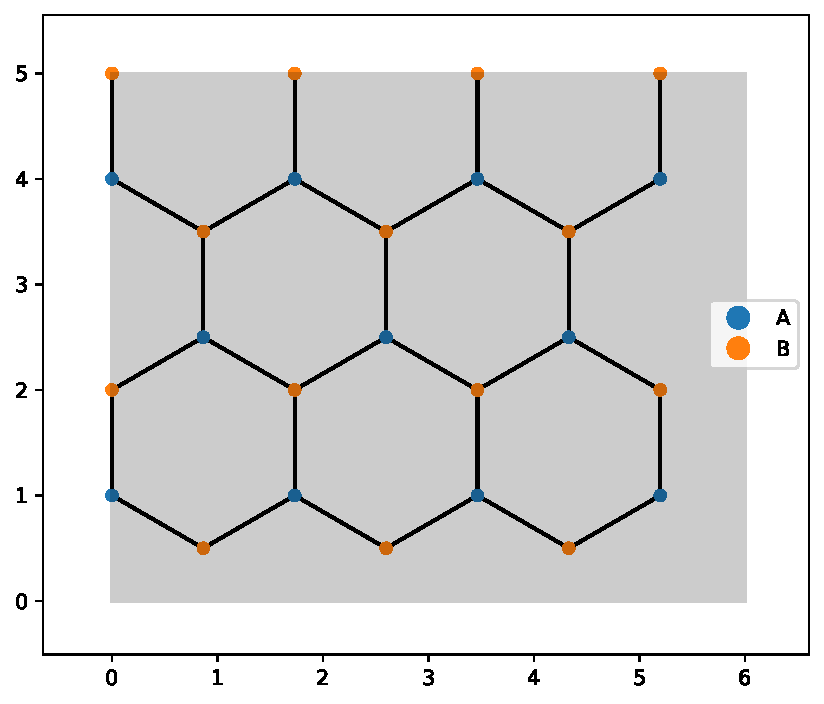
\includegraphics[width=0.7\textwidth]{images/graphene lattice}
    \caption{Graphene lattice structure}
    \label{fig:graphene lattice structure}
\end{figure}

Vectors to the nearest-neighbor \(B_i\) (\(i = 1, 2, 3,\)) atoms from atom \(A\):
\begin{align}
    \vb{\delta}_{AB, 1} = \begin{pmatrix} 0 \\ \frac{a}{\sqrt{3}} \end{pmatrix}, \vb{\delta}_{AB, 2} = \begin{pmatrix} \frac{a}{2} \\ -\frac{a}{2\sqrt{3}} \end{pmatrix}, \vb{\delta}_{AB, 3} = \begin{pmatrix} -\frac{a}{2} \\ -\frac{a}{2\sqrt{3}} \end{pmatrix}
\end{align}

Vectors to the nearest-neighbor \(A_i\) (\(i = 1, 2, 3,\)) atoms from atom \(B\):
\begin{align}
    \vb{\delta}_{BA, 1} = \begin{pmatrix} 0 \\ -\frac{a}{\sqrt{3}} \end{pmatrix}, \vb{\delta}_{BA, 2} = \begin{pmatrix} \frac{a}{2} \\ \frac{a}{2\sqrt{3}} \end{pmatrix}, \vb{\delta}_{BA, 3} = \begin{pmatrix} -\frac{a}{2} \\ \frac{a}{2\sqrt{3}} \end{pmatrix}
\end{align}

The vectors between the Graphene \(\mathrm{A}\) atom and the six neighbours on the same sub lattice can be found by rotating \(\vb{a}_1\) six times by \(\nicefrac{1}{6} * 2\pi = \nicefrac{\pi}{3}\):
\begin{align}
    \vb{\delta}_{AA, 1} &= \vb{a}_1 = \frac{a}{2} \begin{pmatrix} 1 \\ \sqrt{3} \end{pmatrix} = a \begin{pmatrix} \frac{1}{2} \\ \frac{\sqrt{3}}{2} \end{pmatrix} = a \begin{pmatrix} \sin{(\frac{\pi}{6})} \\ \cos{(\frac{\pi}{6})} \end{pmatrix} \\
    \vb{\delta}_{AA, 2} &= a \begin{pmatrix} \sin{(\frac{3\pi}{6})} \\ \cos{(\frac{3\pi}{6})} \end{pmatrix} = a \begin{pmatrix} 1 \\ 0 \end{pmatrix} \\
    \vb{\delta}_{AA, 3} &= a \begin{pmatrix} \sin{(\frac{5\pi}{6})} \\ \cos{(\frac{5\pi}{6})} \end{pmatrix} = a \begin{pmatrix} \frac{1}{2} \\ -\frac{\sqrt{3}}{2} \end{pmatrix} \\
    \vb{\delta}_{AA, 4} &= a \begin{pmatrix} \sin{(\frac{7\pi}{6})} \\ \cos{(\frac{7\pi}{6})} \end{pmatrix} = a \begin{pmatrix} -\frac{1}{2} \\ -\frac{\sqrt{3}}{2} \end{pmatrix} \\
    \vb{\delta}_{AA, 5} &= a \begin{pmatrix} \sin{(\frac{9\pi}{6})} \\ \cos{(\frac{9\pi}{6})} \end{pmatrix} = a \begin{pmatrix} -1 \\ 0 \end{pmatrix} \\
    \vb{\delta}_{AA, 6} &= a \begin{pmatrix} \sin{(\frac{11\pi}{6})} \\ \cos{(\frac{11\pi}{6})} \end{pmatrix} = a \begin{pmatrix} -\frac{1}{2} \\ \frac{\sqrt{3}}{2} \end{pmatrix}
\end{align}

\begin{figure}[htb]
    \centering
    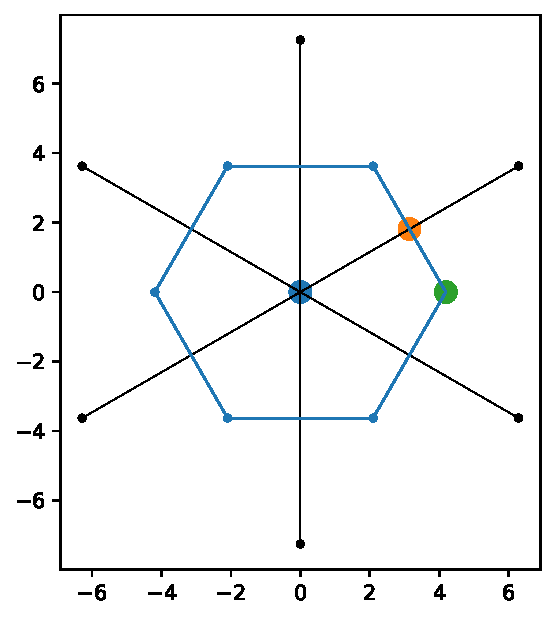
\includegraphics[width=0.5\textwidth]{images/graphene brillouin_zone}
    \caption{Graphene Brillouin Zone}
    \label{fig:graphene Brillouin zone}
\end{figure}

The primitive reciprocal lattice vectors \(\vb{b}_1\), \(\vb{b}_2\) fulfill
\begin{align}
    \vb{a}_1 \cdot \vb{b}_1 &= \vb{a}_2 \cdot \vb{b}_2 = 2\pi \\
    \vb{a}_1 \cdot \vb{b}_2 &= \vb{a}_2 \cdot \vb{b}_1 = 0
    \;,
\end{align}
so we have:
\begin{align}
    \vb{b}_1 &= \frac{2\pi}{a} \begin{pmatrix} 1 \\ \frac{1}{\sqrt{3}} \end{pmatrix} \\
    \vb{b}_2 &= \frac{2\pi}{a} \begin{pmatrix} 1 \\ - \frac{1}{\sqrt{3}} \end{pmatrix}
\end{align}
Points of high symmetry in the Brillouin zone are:
\begin{align}
    \Gamma &= \begin{pmatrix} 0 \\ 0 \end{pmatrix} \\
    \mathrm{M} &= \frac{\pi}{a} \begin{pmatrix} 1 \\ \frac{1}{\sqrt{3}} \end{pmatrix} \\
    \mathrm{K} &= \frac{4\pi}{3 a} \begin{pmatrix} 1 \\ 0 \end{pmatrix}
\end{align}

\section{EG-X Model}\label{sec:eg-x-model}

Graphene lattice and a site X\@.
\begin{figure}[htb]
    \centering
    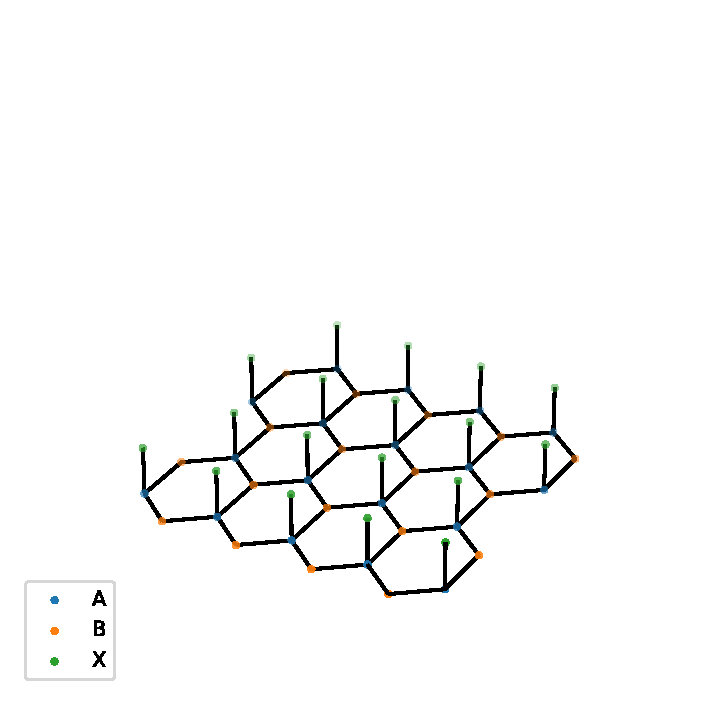
\includegraphics[width=0.5\textwidth]{images/eg-x lattice}
    \caption{EG-X model}
    \label{fig:eg-x model}
\end{figure}
Real-life motivation: layer of graphene on top of a substrate of another material (which provides the additional X atoms).
There is no spin-orbit coupling considered in the model (but when according to Niklas: when mapping to substrates Sn or Pb, it could be necessary (but does not the qualitative result?)).

Without interaction \todo{Spin-orbit coupling, drop second spin index?}:
\begin{align}
    H_0 &= -t_{\mathrm{X}} \sum_{\langle ij \rangle, \sigma \sigma^{\prime}} d_{i, \sigma}^{\dagger} d_{j, \sigma^{\prime}} + \mathrm{h.c.}
    -t_{\mathrm{Gr}} \sum_{\langle ij \rangle, \sigma \sigma^{\prime}} \left(
    c_{i, \sigma}^{(A), \dagger} c_{j, \sigma^{\prime}}^{(B)} +
    c_{j, \sigma^{\prime}}^{(B), \dagger} c_{i, \sigma}^{(A)} + \mathrm{h.c.}
    \right) \\
    &+ V \sum_{i, \sigma \sigma^{\prime}} \left(
    d_{i, \sigma}^{\dagger} c_{i, \sigma^{\prime}}^{(A)} +
    c_{i, \sigma}^{(A), \dagger} d_{i, \sigma^{\prime}}
    \right)
    \label{eq:EG-X model Hamiltonian non-interacting}
\end{align}
with:
\begin{itemize}
    \item \(d\) operators on the X atom
    \item \(c^{(\epsilon)}\) operators on the graphene site (\(\epsilon = A, B\))
    \item \(t_X\) NN hopping for X
    \item \(t_{Gr}\) NN hopping of Gr
    \item \(V\) hybridization between \(\mathrm{X}\) and Graphene \(\mathrm{B}\) sites
\end{itemize}
We can also introduce an onsite Hubbard interaction:
\begin{equation}
    H_{\mathrm{int}} = U_{\mathrm{X}} \sum_{i} d_{i, \uparrow}^{\dagger} d_{i, \downarrow}^{\dagger} d_{i, \downarrow} d_{i, \uparrow}
    + U_{\mathrm{Gr}} \sum_{i, \epsilon=A, B} c_{i, \uparrow}^{(\epsilon) \dagger} c_{i, \downarrow}^{(\epsilon) \dagger} c_{i, \downarrow}^{\epsilon} c_{i, \uparrow}^{\epsilon}
\end{equation}

\subsection{Review: Hubbard model on the honeycomb lattice}\label{subsec:review:-hubbard-model-on-the-honeycomb-lattice}

\todo{Write review for Hubbard model on the honeycomb lattice}

\subsection{Band structure of the non-interacting EG-X model}\label{subsec:band-structure-of-the-non-interacting-eg-x-model}

To treat eq.~\ref{eq:EG-X model Hamiltonian non-interacting}, we first write out the sums over nearest neighbours \(\langle i, j \rangle\) explicitly, writing \(\vb{\delta}_{\mathrm{X}}, \vb{\delta}_{\epsilon}\) (\(\epsilon = A, B\)) for the connections to the nearest neighbours of the \(\mathrm{X}\) atoms and Graphene \(A, B\) sites.
Doing the calculation for the example of the \(\mathrm{X}\) atoms:
\begin{align}
    &-t_{\mathrm{X}} \sum_{\langle ij \rangle, \sigma \sigma^{\prime}} (d_{i, \sigma}^{\dagger} d_{j, \sigma^{\prime}} + d_{j, \sigma}^{\dagger} d_{i, \sigma^{\prime}}) \\
    &= -\frac{t_X}{2} \sum_{i,\sigma, \sigma^{\prime}} \sum_{\delta_{\mathrm{X}}} d_{i, \sigma}^{\dagger} d_{i + \delta_{\mathrm{X}}, \sigma^{\prime}}
    -\frac{t_X}{2} \sum_{j,\sigma, \sigma^{\prime}} \sum_{\delta_{\mathrm{X}}} d_{j, \sigma}^{\dagger} d_{j + \delta_{\mathrm{X}}, \sigma^{\prime}} \\
    &= -t_X \sum_{i,\sigma, \sigma^{\prime}} \sum_{\delta_{\mathrm{X}}} d_{i, \sigma}^{\dagger} d_{i + \delta_{\mathrm{X}}, \sigma^{\prime}}
    \label{eq:EG-X model X atoms nearest neighbours written out}
\end{align}
(The factor \(\nicefrac{1}{2}\) is to account for double counting when going to the sum over all lattice sites \(i\))

Now we can input the discrete Fourier transform (for both graphene and X operators) into eq.~\ref{eq:EG-X model X atoms nearest neighbours written out}
\begin{align}
    c_{i} &= \frac{1}{\sqrt{N}} \sum_{\vb{k}} e^{\iu \vb{k} \vb{r}_{i}} c_{\vb{k}} \\
    c_{i}^{\dagger} &= \frac{1}{\sqrt{N}} \sum_{\vb{k}} e^{-\iu \vb{k} \vb{r}_{i}} c_{\vb{k}}^{\dagger}
\end{align}
with the completeness relation:
\begin{equation}
    \sum_{i} e^{\iu \vb{k} \vb{r}_{i}} e^{-\iu \vb{k}^{\prime} \vb{r}_{i}} = N \delta_{\vb{k}, \vb{k}^{\prime}}
    \;.
\end{equation}
We get:
\begin{align}
    -t_X \frac{1}{N} \sum_{i,\sigma, \sigma^{\prime}} \sum_{\vb{\delta}_{\mathrm{X}}} d_{i, \sigma}^{\dagger} d_{i + \vb{\delta}_{\mathrm{X}}, \sigma^{\prime}}
    &= -t_X \frac{1}{N} \sum_{i,\sigma, \sigma^{\prime}} \sum_{\vb{\delta}_{\mathrm{X}}} \sum_{\vb{k}, \vb{k}^{\prime}} e^{-\iu \vb{k} \vb{r}_i} d_{\vb{k}, \sigma}^{\dagger} e^{\iu \vb{k}^{\prime} \vb{r}_i} e^{\iu \vb{k}^{\prime} \vb{\delta}_{\mathrm{X}}} d_{\vb{k}^{\prime}, \sigma^{\prime}} \\
    &= -t_X \frac{1}{N} \sum_{\vb{k}, \vb{k^{\prime}}, \sigma, \sigma^{\prime}} \sum_{\vb{\delta}_{\mathrm{X}}} d_{\vb{k}, \sigma}^{\dagger}  e^{\iu \vb{k}^{\prime} \vb{\delta}_{\mathrm{X}}} d_{\vb{k}^{\prime}, \sigma^{\prime}} \sum_{i} e^{-\iu \vb{k} \vb{r}_i} e^{\iu \vb{k}^{\prime} \vb{r}_i} \\
    &= -t_X \frac{1}{N} \sum_{\vb{k}, \vb{k^{\prime}}, \sigma, \sigma^{\prime}} \sum_{\vb{\delta}_{\mathrm{X}}} d_{\vb{k}, \sigma}^{\dagger}  e^{\iu \vb{k}^{\prime} \vb{\delta}_{\mathrm{X}}} d_{\vb{k}^{\prime}, \sigma^{\prime}} N \delta_{\vb{k}, \vb{k}^{\prime}} \\
    &= -t_X \sum_{\vb{k}, \sigma, \sigma^{\prime}}  d_{\vb{k}, \sigma}^{\dagger}d_{\vb{k}, \sigma^{\prime}} \sum_{\vb{\delta}_{\mathrm{X}}} e^{\iu \vb{k} \vb{\delta}_{\mathrm{X}}}
\end{align}
The nearest neighbours for \(\mathrm{X}\) atoms are the vectors \(\vb{\delta}_{AA, i}\) from section~\ref{sec:lattice-structure-of-graphene}.
With that, we can calculate:
\begin{align}
    f_{\mathrm{X}} (\vb{k}) &= -t_X \sum_{\vb{\delta}_{\mathrm{X}}} e^{\iu \vb{k} \vb{\delta}_{\mathrm{X}}} \\
    &= -t_X \left( e^{\iu a (\frac{k_x}{2} + \frac{\sqrt{3} k_y}{2})}
    + e^{\iu a k_x}
    + e^{\iu a (\frac{k_x}{2} - \frac{\sqrt{3} k_y}{2})}
    \right. \\
    &+ \left. e^{\iu a (-\frac{k_x}{2} - \frac{\sqrt{3} k_y}{2})}
    + e^{-\iu a k_x}
    + e^{\iu a (-\frac{k_x}{2} + \frac{\sqrt{3} k_y}{2})} \right) \\
    &= -t_X \left( 2 \cos{(a k_x)} + 2 e^{\iu a \frac{\sqrt{3} k_y}{2}} \cos{(\frac{a}{2} k_x)} + 2 e^{-\iu a \frac{\sqrt{3} k_y}{2}} \cos{(\frac{a}{2} k_x)} \right) \\
    &= -2t_X \left( \cos{(a k_x)} + 2 \cos{(\frac{a}{2} k_x)} \cos{(\sqrt{3} \frac{ a}{2} k_y)} \right)
\end{align}
We can do the same for the hopping between Graphene sites, for example :
\begin{align}
    -t_{\mathrm{Gr}} \sum_{\langle ij \rangle, \sigma \sigma^{\prime}} c_{i, \sigma}^{(A), \dagger} c_{j, \sigma^{\prime}}^{(B)}
    &= -t_{\mathrm{Gr}} \sum_{i, \sigma \sigma^{\prime}} \sum_{\vb{\delta}_{AB}} c_{i, \sigma}^{(A), \dagger} c_{i + \vb{\delta}_{AB} , \sigma^{\prime}}^{(B)} \\
    &= -t_{\mathrm{Gr}} \sum_{\vb{k}, \sigma, \sigma^{\prime}}  c_{\vb{k}, \sigma}^{(A) \dagger} c_{\vb{k}, \sigma^{\prime}}^{(B)} \sum_{\vb{\delta}_{AB}} e^{\iu \vb{k} \vb{\delta}_{AB}}
\end{align}
We note
\begin{align}
    \sum_{\vb{\delta}_{AB}} e^{\iu \vb{k} \vb{\delta}_{AB}} = \left( \sum_{\vb{\delta}_{BA}} e^{\iu \vb{k} \vb{\delta}_{BA}} \right)^* = \sum_{\vb{\delta}_{BA}} e^{-\iu \vb{k} \vb{\delta}_{BA}}
\end{align}
and calculate
\begin{align}
    f_{Gr} &= -t_{Gr} \sum_{\vb{\delta}_{AB}} e^{\iu \vb{k} \vb{\delta}_{AB}} \\
    &= -t_{Gr} \left(
    e^{\iu \frac{a}{\sqrt{3}} k_y} +
    e^{\iu \frac{a}{2\sqrt{3}} (\sqrt{3} k_x - k_y)} +
    e^{\iu \frac{a}{2\sqrt{3}} (-\sqrt{3} k_x - k_y)} \right) \\
    &= -t_{Gr} \left(
    e^{\iu \frac{a}{\sqrt{3}} k_y} +
    e^{-\iu \frac{a}{2\sqrt{3}} k_y} \left(
        e^{\iu \frac{a}{2} k_x} + e^{-\iu \frac{a}{2} k_x}
    \right) \right) \\
    &= -t_{Gr} \left(
    e^{\iu \frac{a}{\sqrt{3}} k_y} +
    2 e^{-\iu \frac{a}{2\sqrt{3}} k_y}
    \cos{(\frac{a}{2} k_x)} \right)
\end{align}
All together, we get:
\begin{align}
    H_0 &= \sum_{\vb{k}, \sigma, \sigma^{\prime}} \begin{pmatrix} c_{k, \sigma}^{A, \dagger} & c_{k, \sigma}^{B, \dagger} & d_{k, \sigma}^{\dagger} \end{pmatrix}
    \begin{pmatrix}
        0 & f_{Gr} & V \\
        f_{Gr}^* & 0 & 0 \\
        V & 0 & f_{X}
    \end{pmatrix} \begin{pmatrix} c_{k, \sigma}^{A} \\ c_{k, \sigma}^{B} \\ d_{k, \sigma} \end{pmatrix}
    \label{eq:EG-X Hamiltonian non-interacting matrix}
\end{align}
The band structure for the non-interacting EG-X model is easily obtained by diagonalising the matrix in eq.~\ref{eq:EG-X Hamiltonian non-interacting matrix}.
This was done in fig.~\ref{fig:EG-X model non-interacting bands}.

Values used for calculation:
\begin{itemize}
    \item \(a_0 = 1\)
    \item \(t_{\mathrm{Gr}} = 1\)
    \item \(t_{\mathrm{X}} = 0.01\)
\end{itemize}
\(V\) is the control parameter.
(According to Niklas), a range from \(V = 0.1\) to \(V = 2\) can be mapped onto materials in experiment.

\begin{figure}[t]
    \centering
    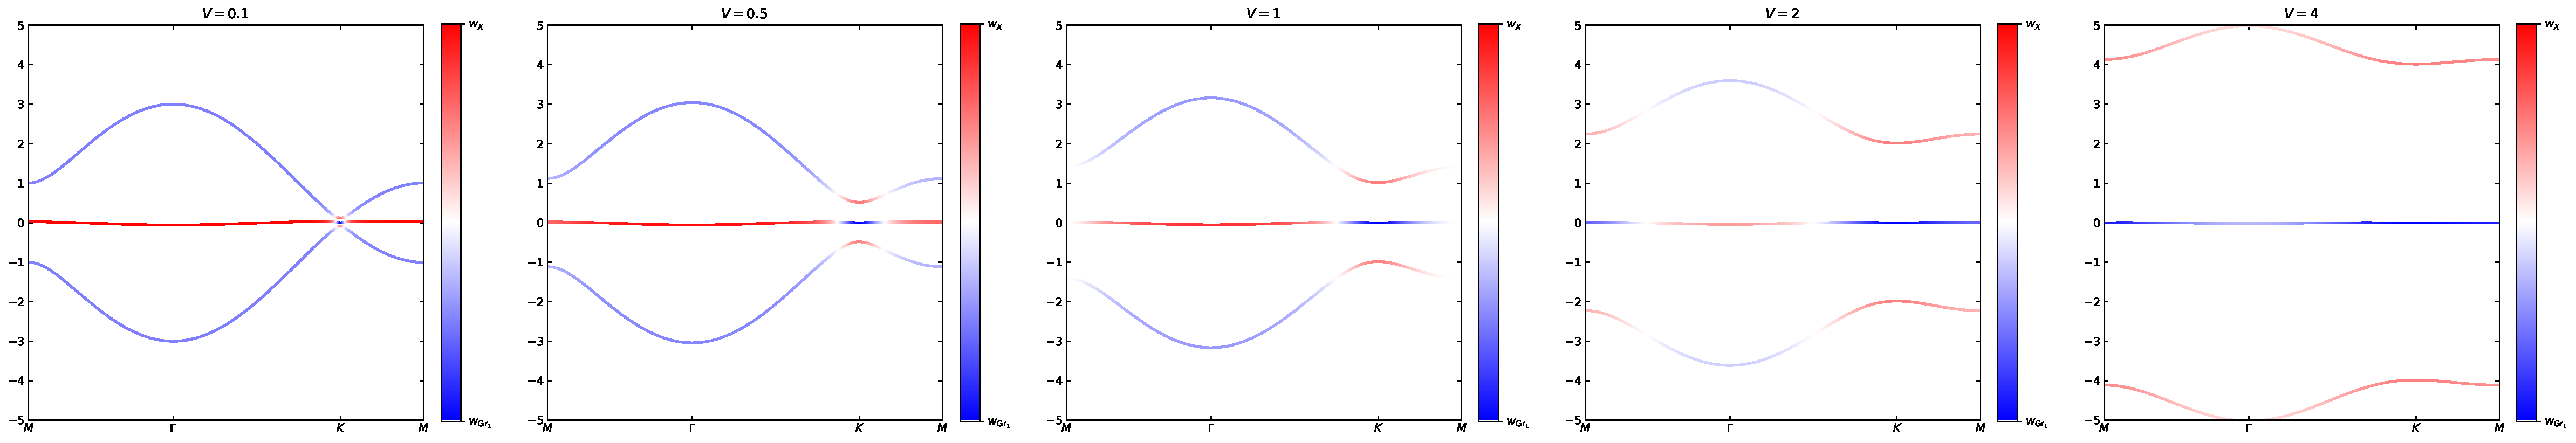
\includegraphics[width=\textwidth]{images/EG_X bands_tGr_1_tX_0.01}
    \caption{Bands of the non-interacting EG-X model. All the bands are spin-degenerate.}
    \label{fig:EG-X model non-interacting bands}
\end{figure}

\section{BCS Theory on the EG-X Model}\label{sec:bcs-theory-on-the-eg-x-model}

\subsection{BdG Hamiltonian}

Define sublattice index
\begin{equation}
    \alpha = 1, 2, 3
\end{equation}
with \(1 \hateq \mathrm{Gr}_1, 2 \hateq \mathrm{Gr}_2, 3 \hateq \mathrm{X}\).
Then we can write the non-interacting term as
\begin{equation}
    H_0 = - \sum_{\langle i, j \rangle, \alpha, \beta, \sigma} \left[\mat{t} \right]_{i\alpha,j\beta} c_{i\alpha}^{\dagger} c_{j\beta}
\end{equation}
with the matrix \todo{Does that make sense?}
\begin{equation}
    \mat{t} = \begin{pmatrix}
                  0 & t_{\mathrm{Gr}} & 0 \\
                  t_{\mathrm{Gr}} & 0 & -V \delta_{ij} \\
                  0 & -V \delta_{ij} & t_{\mathrm{X}} \\
    \end{pmatrix}
\end{equation}

Add chemical potential:
\begin{equation}
    -\mu \sum_{i \alpha \sigma} n_{i \alpha \sigma}
\end{equation}

Also write the interaction part with \(\alpha\) (with changed signs compared to Niklas, to keep in line with papers about the attractive Hubbard model):
\begin{equation}
    H_{int} = - \sum_{i \alpha} U_{\alpha} c_{i\alpha \uparrow}^{\dagger} c_{i\alpha \downarrow}^{\dagger} c_{i\alpha \downarrow} c_{i\alpha \uparrow}
\end{equation}
Fourier transformation:
\begin{equation}
    H_{int} = - \frac{1}{N^2} \sum_{\alpha, \vb{k}_{1, 2, 3, 4}} U_{\alpha} e^{\iu (\vb{k}_1 + \vb{k}_4 - \vb{k}_1 - \vb{k}_3) r_{i \alpha}}  c_{\vb{k}_1 \alpha \uparrow}^{\dagger} c_{\vb{k}_3 \alpha \downarrow}^{\dagger} c_{\vb{k}_2 \alpha \downarrow} c_{\vb{k}_4 \alpha \uparrow}
\end{equation}
Impose zero-momentum pairing: \(\vb{k}_1 + \vb{k}_3 = 0\) and \(\vb{k}_2 + \vb{k}_4 = 0\):
\begin{align}
    H_{int} = - \sum_{\alpha, \vb{k}, \vb{k}^{\prime}} U_{\alpha} c_{\vb{k} \alpha \uparrow}^{\dagger} c_{-\vb{k} \alpha \downarrow}^{\dagger} c_{-\vb{k}^{\prime} \alpha \downarrow} c_{\vb{k}^{\prime} \alpha \uparrow}
\end{align}
Mean-field approximation:
\begin{align}
    H_{int} \approx \sum_{\alpha, \vb{k}} (\Delta_{\alpha} c_{\vb{k} \alpha \uparrow}^{\dagger} c_{-\vb{k} \alpha \downarrow}^{\dagger} + \Delta_{\alpha}^* c_{-\vb{k} \alpha \downarrow} c_{\vb{k} \alpha \uparrow})
\end{align}
with
\begin{align}
    \Delta_{\alpha} &= - U_{\alpha} \sum_{\vb{k}^{\prime}} \braket{c_{-\vb{k}^{\prime} \alpha \downarrow} c_{\vb{k}^{\prime} \alpha \uparrow}} \\
    \Delta_{\alpha}^* &= - U_{\alpha} \sum_{\vb{k}^{\prime}} \braket{c_{\vb{k}^{\prime} \alpha \uparrow}^{\dagger} c_{-\vb{k}^{\prime} \alpha \downarrow}^{\dagger}}
\end{align}
This gives the BCS mean field Hamiltonian:
\begin{align}
    H_{BCS} = \sum_{\vb{k} \alpha \beta \sigma} [H_{0, \sigma} (\vb{k})]_{\alpha \beta} c_{\vb{k} \alpha \sigma}^{\dagger} c_{\vb{k} \beta \sigma}
    -\mu \sum_{\vb{k} \alpha \sigma} n_{\vb{k} \alpha \sigma}
    + \sum_{\alpha, \vb{k}} (\Delta_{\alpha} c_{\vb{k} \alpha \uparrow}^{\dagger} c_{-\vb{k} \alpha \downarrow}^{\dagger} + \Delta_{\alpha}^* c_{-\vb{k} \alpha \downarrow} c_{\vb{k} \alpha \uparrow})
\end{align}
with Nambu spinor
\begin{equation}
    \Psi_{\vb{k}} =
    \begin{pmatrix}
        c_{1, \vb{k} \uparrow} \\
        c_{2, \vb{k} \uparrow} \\
        c_{3, \vb{k} \uparrow} \\
        c_{1, -\vb{k} \downarrow}^{\dagger} \\
        c_{2, -\vb{k} \downarrow}^{\dagger} \\
        c_{3, -\vb{k} \downarrow}^{\dagger} \\
    \end{pmatrix}
\end{equation}
we have:
\begin{equation}
    H_{MF} = \sum_{\vb{k}} \Psi_{\vb{k}}^{\dagger} \mathcal{H} (\vb{k}) \Psi_{\vb{k}}
\end{equation}
with
\begin{equation}
    \mathcal{H} (\vb{k}) =
    \begin{pmatrix}
        H_{0, \uparrow} (\vb{k}) - \mu & \Delta \\
        \Delta^{\dagger} & - H_{0, \downarrow}^* (-\vb{k}) + \mu
    \end{pmatrix}
\end{equation}
with \(H_{0, \sigma}\) being the F.T. of the kinetic term and \(\Delta = diag(\Delta_1, \Delta_2, \Delta_3)\).

\subsection{BdG Hamiltonian in band basis}

Use transformation
\begin{equation}
    c_{\vb{k} \alpha \sigma}^{\dagger} = \sum_{n} [\mat{G}]_{\alpha n}^* d_{n \vb{k} \sigma}^{\dagger}
\end{equation}
where the columns are made up of the eigenvectors of \(\mat{H}_{0, \sigma}\) for a given \(\vb{k}\):
\begin{equation}
    \mat{G} = 
    \begin{pmatrix}
        \vb{G}_1 & \vb{G}_2 & \vb{G}_3
    \end{pmatrix}
\end{equation}

with that:
\begin{equation}
    \mat{G}^{\dagger}_{\sigma} (\vb{k}) \mat{H}_{0, \sigma} (\vb{k}) \mat{G}_{\sigma} (\vb{k}) =
    \begin{pmatrix}
        \epsilon_1 & 0 & 0 \\
        0 & \epsilon_2 & 0 \\
        0 & 0 & \epsilon_3
    \end{pmatrix}
\end{equation}
So the kinetic part of the BdG Hamiltonian becomes:
\begin{align}
    &\sum_{\vb{k} \alpha \beta \sigma} [H_{0, \sigma} (\vb{k})]_{\alpha \beta}
    \sum_{n} [\mat{G} (\vb{k})]_{\alpha n}^* d_{n \vb{k} \sigma}^{\dagger}
    \sum_{m} [\mat{G} (\vb{k})]_{\beta m} d_{m \vb{k} \sigma}
    -\mu \sum_{\vb{k} \alpha \sigma} n_{n \vb{k} \sigma} \\
    &= \sum_{m n \vb{k} \sigma} d_{n \vb{k} \sigma}^{\dagger} d_{m \vb{k} \sigma}
   \sum_{\alpha \beta} [\mat{G} (\vb{k})]_{\alpha n}^* [H_{0, \sigma} (\vb{k})]_{\alpha \beta} [\mat{G} (\vb{k})]_{\beta m}
    -\mu \sum_{\vb{k} \alpha \sigma} n_{n \vb{k} \sigma} \\
    &= \sum_{m n \vb{k} \sigma} d_{n \vb{k} \sigma}^{\dagger} d_{m \vb{k} \sigma} \epsilon_{n} \delta_{n m}
    -\mu \sum_{\vb{k} \alpha \sigma} n_{n \vb{k} \sigma} \\
    &= \sum_{n \vb{k} \sigma} \epsilon_{n} d_{n \vb{k} \sigma}^{\dagger} d_{n \vb{k} \sigma}
    -\mu \sum_{\vb{k} \alpha \sigma} n_{n \vb{k} \sigma} \\
    &\eqqcolon \sum_{n \vb{k} \sigma} \xi_{\vb{k}} d_{n \vb{k} \sigma}^{\dagger} d_{n \vb{k} \sigma}
\end{align}
with \(\xi_{\vb{k}} \coloneqq \epsilon_{\vb{k}} - \mu\).
The pairing terms become (I set \(n = m\) here, which seems only sensible, but I dont have a real reason why?):
\begin{align}
    \sum_{\vb{k} \alpha} \Delta_{\alpha} c_{\vb{k} \alpha \uparrow}^{\dagger} c_{-\vb{k} \alpha \downarrow}^{\dagger}
    &= \sum_{\vb{k} \alpha} \Delta_{\alpha} \sum_n [\mat{G}_{\uparrow} (\vb{k})]_{\alpha n}^* d_{n \vb{k} \uparrow}^{\dagger} \sum_m [\mat{G}_{\downarrow} (-\vb{k})]_{\beta m}^* d_{m -\vb{k} \downarrow}^{\dagger} \\
    &= -\sum_{n \vb{k}} \Delta_n d_{n \vb{k} \uparrow}^{\dagger} d_{n -\vb{k} \downarrow}^{\dagger}
\end{align}
with gap \(\Delta_n (\vb{k}) = -\sum_{\alpha} [\mat{G}_{\uparrow} (\vb{k})]_{\alpha n}^* \Delta_{\alpha} [\mat{G}_{\downarrow} (-\vb{k})]_{\alpha n}^*\) for band \(n\).
\begin{align}
    \sum_{\vb{k} \alpha} \Delta_{\alpha}^* c_{-\vb{k} \alpha \downarrow} c_{\vb{k} \alpha \uparrow}
    &= -\sum_{n \vb{k}} \Delta_n^* d_{n -\vb{k} \downarrow} d_{n \vb{k} \uparrow}
\end{align}

So the BdG Hamiltonian is:
\begin{align}
    H_{BdG} = \sum_{n \vb{k} \sigma} \xi_{\vb{k}} d_{n \vb{k} \sigma}^{\dagger} d_{n \vb{k} \sigma}
    -\sum_{n \vb{k}} (\Delta_n^* d_{n -\vb{k} \downarrow} d_{n \vb{k} \uparrow} + \Delta_n d_{n \vb{k} \uparrow}^{\dagger} d_{n -\vb{k} \downarrow}^{\dagger})
\end{align}

\subsection{Self-consistent calculation of the superconducting gaps}

Compare~\cite[ch. 10]{Bruus_Flensberg_2004}.
Notable here: Multiple bands, and the gaps in each band depend in a complicated manner on the parameters \(U_{\alpha}\) and the orbital Green's functions.

Define normal Green's function:
\begin{equation}
    \mathcal{G}_{n\uparrow n\uparrow} (\vb{k}, \tau) = -\braket{T_{\tau} d_{n \vb{k} \uparrow} (\tau) d_{n \vb{k} \uparrow}^{\dagger} (0)}
\end{equation}
Anomalous Green's function:
\begin{equation}
    \mathcal{F}_{n\downarrow n\uparrow} (\vb{k}, \tau) = -\braket{T_{\tau} d_{n -\vb{k} \downarrow} (\tau) d_{n \vb{k} \uparrow}^{\dagger} (0)}
\end{equation}

Equations of motion (Heisenberg equation), follow~\cite[ch. 17]{Bruus_Flensberg_2004}:
\begin{align}
    \pdif{\tau} \mathcal{G}_{n\uparrow n\uparrow} (\vb{k}, \tau) &= -\delta (\tau) + \braket{T_{\tau} \left[d_{n \vb{k} \uparrow}, H_{BdG}\right] (\tau) d_{n \vb{k} \uparrow}^{\dagger} (0)} \\
    \pdif{\tau} \mathcal{F}_{n\downarrow n\uparrow} (\vb{k}, \tau) &= \braket{T_{\tau} \left[d_{n -\vb{k} \downarrow}, H_{BdG}\right] (\tau) d_{n \vb{k} \uparrow}^{\dagger} (0)}
\end{align}

To calculate the commutators, use the relation (for operators \(A\), \(B\), \(C\)):
\begin{align}
    [A, BC] = ABC - BCA = (\{A, B\} - BA) C - B(\{C, A\} - AC)
\end{align}

\begin{align}
    \left[ d_{n -\vb{k} \downarrow}^{\dagger}, H_0 \right]
    &= \sum_{n^{\prime} \vb{k}^{\prime} \sigma^{\prime}} \xi_{n^{\prime} \vb{k}^{\prime}} \left[ d_{n -\vb{k} \downarrow}^{\dagger}, d_{n^{\prime} \vb{k}^{\prime} \sigma^{\prime}}^{\dagger} d_{n^{\prime} \vb{k}^{\prime} \sigma^{\prime}} \right] \\
    &= \sum_{n^{\prime} \vb{k}^{\prime} \sigma^{\prime}} \xi_{n^{\prime} \vb{k}^{\prime}}
    \left(
        \{d_{n -\vb{k} \downarrow}^{\dagger}, d_{n^{\prime} \vb{k}^{\prime} \sigma^{\prime}}^{\dagger} \} - d_{n^{\prime} \vb{k}^{\prime} \sigma^{\prime}}^{\dagger} d_{n -\vb{k} \downarrow}^{\dagger}
    \right) d_{n^{\prime} \vb{k}^{\prime} \sigma^{\prime}} \\
    &- d_{n^{\prime} \vb{k}^{\prime} \sigma^{\prime}}^{\dagger}
    \left(
        \{ d_{n^{\prime} \vb{k}^{\prime} \sigma^{\prime}}, d_{n -\vb{k} \downarrow}^{\dagger} \} - d_{n -\vb{k} \downarrow}^{\dagger} d_{n^{\prime} \vb{k}^{\prime} \sigma^{\prime}}
    \right) \\
    &= \sum_{n^{\prime} \vb{k}^{\prime} \sigma^{\prime}} \xi_{n^{\prime} \vb{k}^{\prime}}
    \left(- d_{n^{\prime} \vb{k}^{\prime} \sigma^{\prime}}^{\dagger} d_{n -\vb{k} \downarrow}^{\dagger} d_{n^{\prime} \vb{k}^{\prime} \sigma^{\prime}}
    - d_{n^{\prime} \vb{k}^{\prime} \sigma^{\prime}}^{\dagger}
    \delta_{n^{\prime} \vb{k}^{\prime} \sigma^{\prime}, n -\vb{k} \uparrow}
    + d_{n^{\prime} \vb{k}^{\prime} \sigma^{\prime}}^{\dagger} d_{n -\vb{k} \downarrow}^{\dagger} d_{n^{\prime} \vb{k}^{\prime} \sigma^{\prime}} \right) \\
    &= - \xi_{n \vb{k}} d_{n \vb{k} \uparrow}^{\dagger}
\end{align}

\begin{align}
    &\left[d_{n -\vb{k} \downarrow}, -\sum_{m \vb{k}^{\prime}} \Delta_{m}^* d_{m -\vb{k}^{\prime} \downarrow} d_{m \vb{k}^{\prime} \uparrow} \right] \\
    &= -\sum_{m \vb{k}^{\prime}} \Delta_{m}^*
    \left(\{d_{n -\vb{k} \downarrow}, d_{m -\vb{k}^{\prime} \downarrow}\} - d_{m -\vb{k}^{\prime} \downarrow} d_{n -\vb{k} \downarrow} \right) d_{m \vb{k}^{\prime} \uparrow} \\
    &- d_{m -\vb{k}^{\prime} \downarrow} \left(\{ d_{m \vb{k}^{\prime} \uparrow}, d_{n -\vb{k} \downarrow}\} - d_{n -\vb{k} \downarrow} d_{m \vb{k}^{\prime} \uparrow} \right) \\
    &= -\sum_{m \vb{k}^{\prime}} \Delta_{m}^* \left( \delta_{n -\vb{k} \downarrow, m -\vb{k}^{\prime} \downarrow} - d_{m -\vb{k}^{\prime} \downarrow} d_{n -\vb{k} \downarrow} \right) d_{m \vb{k}^{\prime} \uparrow} + d_{m -\vb{k}^{\prime} \downarrow} d_{n -\vb{k} \downarrow} d_{m \vb{k}^{\prime} \uparrow} \\
    &= - \Delta_n^* d_{n \vb{k} \uparrow}
\end{align}

\begin{align}
    \pdif{\tau} \mathcal{F}_{n\downarrow n\uparrow} (\vb{k}, \tau) &=
    -\xi_{n \vb{k}} \braket{T_{\tau} (d_{n -\vb{k} \downarrow}^{\dagger} (\tau) d_{n \vb{k} \uparrow}^{\dagger} (0))} - \Delta_n^* \braket{T_{\tau} (d_{n \vb{k} \uparrow} (\tau) d_{n \vb{k} \uparrow}^{\dagger} (0))} \\
    &= \xi_{n \vb{k}} \mathcal{F}_{n \downarrow n \uparrow} (\vb{k}, \tau) + \Delta_{n}^* \mathcal{G}_{n\uparrow n\uparrow} (\vb{k}, \tau)
\end{align}

Similarly:
\begin{align}
    \left[ d_{n -\vb{k} \uparrow}, H_0 \right]
    &= \sum_{n^{\prime} \vb{k}^{\prime} \sigma^{\prime}} \xi_{n^{\prime} \vb{k}^{\prime}} \left[ d_{n -\vb{k} \downarrow}^{\dagger}, d_{n^{\prime} \vb{k}^{\prime} \sigma^{\prime}}^{\dagger} d_{n^{\prime} \vb{k}^{\prime} \sigma^{\prime}} \right] \\
    &= \xi_{n} d_{n \vb{k} \uparrow}^{\dagger}
\end{align}
\begin{align}
    &\left[d_{n -\vb{k} \uparrow}, -\sum_{m \vb{k}^{\prime}} \Delta_{m} d_{m -\vb{k}^{\prime} \uparrow}^{\dagger} d_{m -\vb{k}^{\prime} \downarrow}^{\dagger} \right] \\
    &= - \Delta_n d_{n -\vb{k} \downarrow}^{\dagger}
\end{align}

\begin{align}
    \pdif{\tau} \mathcal{G}_{n \uparrow n \uparrow} (\vb{k}, \tau) &=
    -\delta(\tau) + \xi_{n \vb{k}} \braket{T_{\tau} d_{n \vb{k} \uparrow} (\tau) d_{n \vb{k} \uparrow}^{\dagger}} - \Delta_n \braket{T_{\tau} d_{n -\vb{k} \downarrow} (\tau) d_{n \vb{k} \uparrow}^{\dagger} (0)} \\
    &= -\delta(\tau) - \xi_{n \vb{k}} \mathcal{G}_{n \uparrow n \uparrow} (\vb{k}, \tau) + \Delta_{n} \mathcal{F}_{n\downarrow n\uparrow} (\vb{k}, \tau) \\
\end{align}

All in all:
\begin{align}
    \pdif{\tau} \mathcal{G}_{n \uparrow n \uparrow} (\vb{k}, \tau) &= -\delta(\tau) - \xi_{n \vb{k}} \mathcal{G}_{n \uparrow n \uparrow} (\vb{k}, \tau) + \Delta_{n} \mathcal{F}_{n\downarrow n\uparrow} (\vb{k}, \tau) \\
    \pdif{\tau} \mathcal{F}_{n \downarrow n \uparrow} (\vb{k}, \tau) &= \xi_{n \vb{k}} \mathcal{F}_{n \downarrow n \uparrow} (\vb{k}, \tau) + \Delta_{n}^* \mathcal{G}_{n\uparrow n\uparrow} (\vb{k}, \tau)
\end{align}
Fourier transform:
\begin{align}
    (-\iu \omega_n + \xi_{n \vb{k}}) \mathcal{G}_{n \uparrow n \uparrow} (\vb{k}, \iu \omega_n) &= -1 + \Delta_{n} \mathcal{F}_{n\downarrow n\uparrow} (\vb{k}, \iu \omega_n) \\
    (-\iu \omega_n - \xi_{n \vb{k}}) \mathcal{F}_{n \downarrow n \uparrow} (\vb{k}, \iu \omega_n) &= \Delta_{n}^* \mathcal{G}_{n\uparrow n\uparrow} (\vb{k}, \iu \omega_n)
\end{align}
This algebraic expression can be easily solved:
\begin{align}
    (-\iu \omega_n - \xi_{n \vb{k}}) \mathcal{F}_{n \downarrow n \uparrow} (\vb{k}, \iu \omega_n) &= \frac{\Delta_{n}^*}{-\iu \omega_n + \xi_{n \vb{k}}} (-1 + \Delta_{n} \mathcal{F}_{n\downarrow n\uparrow} (\vb{k}, \iu \omega_n))
\end{align}
\begin{align}
    (-\iu \omega_n - \xi_{n \vb{k}} - \frac{\vert\Delta_{n}\vert^2}{-\iu \omega_n + \xi_{n \vb{k}}}) \mathcal{F}_{n \downarrow n \uparrow} (\vb{k}, \iu \omega_n) &= \frac{-\Delta_{n}^*}{-\iu \omega_n + \xi_{n \vb{k}}} \\
    (\frac{(-\iu \omega_n - \xi_{n \vb{k}} )(-\iu \omega_n + \xi_{n \vb{k}}) - \vert\Delta_{n}\vert^2}{-\iu \omega_n + \xi_{n \vb{k}}}) \mathcal{F}_{n \downarrow n \uparrow} (\vb{k}, \iu \omega_n) &= \frac{-\Delta_{n}^*}{-\iu \omega_n + \xi_{n \vb{k}}}
\end{align}
\begin{align}
    \mathcal{F}_{n \downarrow n \uparrow} (\vb{k}, \iu \omega_n) &= \frac{-\Delta_{n}^*}{(-\iu \omega_n - \xi_{n \vb{k}} )(-\iu \omega_n + \xi_{n \vb{k}}) - \vert\Delta_{n}\vert^2} \\
    &= \frac{-\Delta_{n}^*}{(\iu \omega_n)^2 - \xi_{n \vb{k}}^2 - \vert\Delta_{n}\vert^2} \\
    &= \frac{-\Delta_{n}^*}{(\iu \omega_n)^2 - E_{n \vb{k}}}
\end{align}
\begin{align}
    (-\iu \omega_n + \xi_{n \vb{k}}) \mathcal{G}_{n \uparrow n \uparrow} (\vb{k}, \iu \omega_n) &= -1 + \frac{-\vert\Delta_{n}\vert^2}{(\iu \omega_n)^2 - \xi_{n \vb{k}}^2 - \vert\Delta_{n}\vert^2} \\
    &= \frac{-(\iu \omega_n)^2 + \xi_{n \vb{k}}^2 + \vert\Delta_{n}\vert^2 -\vert\Delta_{n}\vert^2}{(\iu \omega_n)^2 - \xi_{n \vb{k}}^2 - \vert\Delta_{n}\vert^2} \\
    &= \frac{-(\iu \omega_n)^2 + \xi_{n \vb{k}}^2}{(\iu \omega_n)^2 - \xi_{n \vb{k}}^2 - \vert\Delta_{n}\vert^2} \\
    &= \frac{(\iu \omega_n + \xi_{n \vb{k}})(-\iu \omega_n + \xi_{n \vb{k}})}{(\iu \omega_n)^2 - \xi_{n \vb{k}}^2 - \vert\Delta_{n}\vert^2}
\end{align}
\begin{align}
    \mathcal{G}_{n \uparrow n \uparrow} (\vb{k}, \iu \omega_n) &= \frac{\iu \omega + \xi_{n \vb{k}}}{(\iu \omega_n)^2 - \xi_{n \vb{k}}^2 - \vert\Delta_{n}\vert^2} \\
    &= \frac{\iu \omega + \xi_{n \vb{k}}}{(\iu \omega_n)^2 - E_{n \vb{k}}}
\end{align}
with the energies \(E_{n \vb{k}} = \pm \sqrt{\xi_{n \vb{k}}^2 + \vert\Delta_{n}\vert^2}\).

To calculate the band gap in band \(n\):
\begin{align}
    \Delta_n (\vb{k}) &= -\sum_{\alpha} [G_{k \uparrow}]_{\alpha n}^* \Delta_{\alpha} [G_{-k \downarrow}]_{\alpha n}^* \\
    &= \sum_{\alpha \vb{k}^{\prime}} U_{\alpha} [G_{k \uparrow}]_{\alpha n}^* \braket{c_{-k^{\prime} \alpha \downarrow} c_{k^{\prime} \alpha \uparrow}} [G_{-k \downarrow}]_{\alpha n}^* \\
    &= \sum_{\alpha \vb{k}^{\prime}} U_{\alpha} [G_{k \uparrow}]_{\alpha n}^* [G_{-k \downarrow}]_{\alpha n}^* \sum_{m} [G_{-k^{\prime} \downarrow}]_{\alpha m} [G_{k^{\prime} \uparrow}]_{\alpha m} \braket{d_{-k^{\prime} m \downarrow} d_{k^{\prime} m \uparrow}}
\end{align}
Can now use \(\mathcal{F}\) and fourier-transform:
\begin{align}
    \braket{d_{-k^{\prime} m \downarrow} d_{k^{\prime} m \uparrow}} &= \mathcal{F}_{m \downarrow m \uparrow}^* (\vb{k}^{\prime}, \tau = 0^+) \\
    &= \frac{1}{\beta} \sum_{\iu \omega_n} e^{-\iu \omega_n 0^+} \mathcal{F}_{m \downarrow m \uparrow}^* (\vb{k}^{\prime}, \iu \omega_n)
\end{align}
The summation over the Matsubara frequencies can be solved via the Residue theorem (the poles \(z_0\) of \(\mathcal{F}\) are the energies \(\pm E_{m \vb{k}}\)):
\begin{align}
    &\frac{1}{\beta} \sum_{\iu \omega_n} e^{-\iu \omega_n 0^+} \mathcal{F}_{m \downarrow m \uparrow}^* (\vb{k}^{\prime}, \iu \omega_n) \\
    &= \sum_{z_0 \mathrm{poles of} \mathcal{F}} e^{-z_0 0^+} n_{F} (z_0) Res_{z_0} \mathcal{F}_{m \downarrow m \uparrow}^*  (\vb{k}^{\prime}, z_0) \\
    &= e^{-E_{m \vb{k}} 0^+} n_{F} (E_{m \vb{k}}) Res_{E_{m \vb{k}}} \frac{-\Delta_{m}}{(\iu \omega_n)^2 - E_{m \vb{k}}}
    + e^{E_{m \vb{k}} 0^+} n_{F} (-E_{m \vb{k}}) Res_{-E_{m \vb{k}}} \frac{-\Delta_{m}}{(\iu \omega_n)^2 - E_{m \vb{k}}}
\end{align}
with residue:
\begin{equation}
    Res_{E_{m \vb{k}}} \frac{1}{(\iu \omega_n)^2 - z_0^2} = \frac{1}{\pdif{z}\vert_{z_0 = E_{m \vb{k}}} ((\iu \omega)^2 - z_0^2)} = \frac{1}{2 E_{m \vb{k}}}
\end{equation}
So we have
\begin{align}
    \braket{d_{-k^{\prime} m \downarrow} d_{k^{\prime} m \uparrow}} &= -\Delta_m \left(\frac{n_F (E_{m \vb{k}})}{2 E_{m \vb{k}}} - \frac{n_F (-E_{m \vb{k}})}{2 E_{m \vb{k}}}\right)
\end{align}
The \(n_F\) term can be written as:
\begin{align}
    n_F(E_{m \vb{k}^{\prime}}) - n_F(-E_{m \vb{k}^{\prime}}) &= \frac{1}{e^{\beta E_{m \vb{k}^{\prime}}} + 1} - \frac{1}{e^{-\beta E_{m \vb{k}^{\prime}}} + 1} \\
    &= \frac{e^{-\frac{1}{2} \beta E_{m \vb{k}^{\prime} }}}{e^{-\frac{1}{2} \beta E_{m \vb{k}^{\prime}}}} \frac{1}{e^{\beta E_{m \vb{k}^{\prime}}} + 1} - \frac{e^{\frac{1}{2} \beta E_{m \vb{k}^{\prime}}}}{e^{\frac{1}{2} \beta E_{m \vb{k}^{\prime}}}} \frac{1}{e^{-\beta E_{m \vb{k}^{\prime}}} + 1} \\
    &= \frac{e^{-\frac{1}{2} \beta E_{m \vb{k}^{\prime}}} - e^{\frac{1}{2} \beta E_{m \vb{k}^{\prime}}}}{e^{\frac{1}{2} \beta E_{m \vb{k}^{\prime}}} + e^{-\frac{1}{2} \beta E_{m \vb{k}^{\prime} }}} \\
    &= -\tanh{(\frac{\beta E_{m \vb{k}^{\prime}}}{2})}
\end{align}
This results in the self-concistency equation for the gap:
\begin{align}
    \Delta_n (\vb{k}) = \sum_{\alpha m \vb{k}^{\prime}} U_{\alpha} [G_{k \uparrow}]_{\alpha n}^* [G_{-k \downarrow}]_{\alpha n}^* [G_{-k^{\prime} \downarrow}]_{\alpha m} [G_{k^{\prime} \uparrow}]_{\alpha m} \Delta_{m} (\vb{k}^{\prime}) \frac{\tanh{(\frac{\beta E_{m \vb{k}^{\prime}}}{2})}}{2 E_{m \vb{k}^{\prime}}}
\end{align}
Using time-reversal symmetry \([G_{-\vb{k} \downarrow}]_{\alpha m}^* = [G_{\vb{k} \uparrow}]_{\alpha m}\) this expression gets a bit simpler:
\begin{align}
    \Delta_n (\vb{k}) = \sum_{\alpha m \vb{k}^{\prime}} U_{\alpha} \vert[G_{k \uparrow}]_{\alpha n} \vert^2 \vert[G_{k^{\prime} \uparrow}]_{\alpha m} \vert^2 \Delta_{m} (\vb{k}^{\prime}) \frac{\tanh{(\frac{\beta E_{m \vb{k}^{\prime}}}{2})}}{2 E_{m \vb{k}^{\prime}}}
\end{align}

\subsection{Computational Implementation}

Use scipys \href{https://docs.scipy.org/doc/scipy/reference/generated/scipy.optimize.fixed_point.html}{\texttt{fixed\_point}} solver to solve the gap equation self-consistently.

Flatten \(\Delta_n (\vb{k})\) the following way, to put it into the solver (\(\vb{k}\) discretized in some way):
\begin{equation}
    x = \begin{pmatrix}
        \Re{(\Delta_1 (\vb{k}_1))} \\
        \Re{(\Delta_1 (\vb{k}_2))} \\
        \vdots \\
        \Re{(\Delta_2(\vb{k}_1))} \\
        \vdots \\
        \Re{(\Delta_3(\vb{k}_1))} \\
        \vdots \\
        \Im{(\Delta_1(\vb{k}_1))} \\
        \vdots \\
        \Im{(\Delta_2(\vb{k}_1))} \\
        \vdots \\
        \Im{(\Delta_3(\vb{k}_1))} \\
        \vdots \\
    \end{pmatrix}
\end{equation}
so that accessing a certain element takes the form:
\begin{align}
    \Re{\Delta_n (\vb{k})} &= x\left[\mathrm{index}(\vb{k}) + \frac{\mathrm{len}(x) \cdot n}{6} \right] \\
    \Im{\Delta_n (\vb{k})} &= x\left[\mathrm{index}(\vb{k}) + \frac{\mathrm{len}(x) \cdot n}{6} + \frac{1}{2} \mathrm{len}(x) \right]
\end{align}

\end{document}


\chapter{Green's Function Formalism}\label{ch:green's-function-formalism}

Source: \cite{Bruus_Flensberg_2004}

From TRIQS tutorial:
As you can see, the behavior of the imaginary part is very different for the two values of $U$. When
$U$ is small, the system is a metal and the imaginary part extrapolated to zero goes to a finite value.
Instead, for large $U$, the system is a Mott insulator and the imaginary part goes to zero. The reason
is that the extrapolation to zero is directly proportional to the density of states at the chemical
potential. If the system is gapped, the density is zero; if the system is a metal, there is spectral
weight and the density is finite. Therefore, even on the Matsubara axis, one has a way to decide if the
system is metallic or not.


Most general non-interacting electronic Hamiltonian in second quantization:
\begin{equation}
    H_0 = \sum_{i, j, \sigma}
\end{equation}
with lattice coordinates \(i, j\) and spin \(\sigma\).

\todo{Greens functions introduction (Bruus Flensberg or Coleman or something)}

\todo{Show how Green's functions can be used to describe many-body effects -> Spectral function, self-energy}

One particle Green's function (many-body object, coming from the Hubbard model):
\begin{equation}
    G(\vb{k}, \iu \omega_n) = \frac{1}{\iu \omega_n + \mu - \epsilon_{\vb{k}} - \Sigma(\vb{k}, \iu \omega_n)}
\end{equation}
with the self energy \(\Sigma(\iu \omega_n)\) coming from the solution of the effect on-site problem:

The Dyson equation
\begin{equation}
    G(\vb{k}, \iu \omega_n) = \left( G_0 (\vb{k}, \iu \omega_n) - \Sigma(\vb{k}, \iu \omega_n)\right)^{-1}
\end{equation}
relates the non-interacting Greens function \(G_0 (\vb{k}, \iu \omega_n)\) and the fully-interacting Greens function \(G (\vb{k}, \iu \omega_n)\) (inversion of a matrix!).

\todo{Add citations for: exact limit in infinite dimension, Anderson impurity model}

\todo{Add Mott transition as an achievement}

\todo{Add other achievements?}




\documentclass[../main.tex]{subfiles}
\graphicspath{{\subfix{../images/}}, {\subfix{../}}}

\begin{document}
\chapter{Dynamical Mean-Field Theory}\label{ch:dynamical-mean-field-theory}

\section{Green's Function Formalism}

Following~\cite{bruusManyBodyQuantumTheory2004}

Green's functions: method to encode influence of many-body effects on propagation of particles in a system.

Have different kinds of Green's functions, for example the retarded Green's function:
\begin{equation}
	G^R (\vb{r}\sigma t, \vb{r}^{\prime} \sigma^{\prime} t^{\prime}) = -\iu \Theta(t- t^{\prime}) \braket{ \{c_{\vb{r} \sigma} (t), c_{\vb{r} \sigma}^{\dagger} (t^{\prime})\}}
\end{equation}
They give the amplitude of a particle inserted at point \(\vb{r}^{\prime}\) at time \(t^{\prime}\) to propagate to position \(\vb{r}\) at time \(t\).
For time-independent Hamiltonians and systems in equilibrium, the GFs only depend on time differences:
\begin{equation}
	G^R (\vb{r}\sigma t, \vb{r}^{\prime} \sigma^{\prime} t^{\prime}) = G^R (\vb{r} \sigma, \vb{r}^{\prime} \sigma^{\prime}, t - t^{\prime})
\end{equation}
So we can take \(t^{\prime} = 0\) and consider \(t\) as the only free variable:
\begin{equation}
	G^R (\vb{r}\sigma, \vb{r}^{\prime} \sigma^{\prime}, t) = -\iu \Theta(t) \braket{ \{c_{\vb{r} \sigma} (t), c_{\vb{r} \sigma}^{\dagger} (0)\}}
\end{equation}
In a translation invariant system: can use \(\vb{k}\) as a natural basis set:
\begin{equation}
	G^R (\vb{k}, \sigma, \sigma^{\prime} t) = -\iu \Theta(t- t^{\prime}) \braket{ \{c_{\vb{k} \sigma} (t), c_{\vb{k} \sigma^{\prime}}^{\dagger} (0)\}}
\end{equation}
Define Fourier-transform:
\begin{equation}
	G^R (\vb{k}, \sigma, \sigma^{\prime}, \omega) = \int_{-\infty}^{\infty} \odif{t} G^R (\vb{k}, \sigma, \sigma^{\prime} t)
\end{equation}
Can define the spectral function from this:
\begin{equation}
	A(\vb{k} \sigma, \omega) = -2 \Im G^R (\vb{k} \sigma, \omega)
\end{equation}
Looking at the diagonal elements of \(G^R\) here.
The spectral function can be thought of as the energy resolution of a particle with energy \(\omega\).
This mean, for non-interacting systems, the spectral function is a delta-function around the single-particle energies:
\begin{equation}
	A_0 (\vb{k} \sigma, \omega) = 2\pi \delta (\omega - \epsilon_{\vb{k} \sigma})
\end{equation}
For interacting systems this is not true, but \(A\) can still be peaked.

\todo{Show GFs can be related to observables}

Mathematical technique to calculate retarded GFs involves defining GFs on imaginary times \gls{imaginary time}:
\begin{equation}
	t \to -\iu \tau
\end{equation}
where \(\tau\) is real and has the dimension time.
This enables the simultaneous expansion of exponential \(e^{-\beta H}\) coming from the thermodynamic average and \(e^{-\iu H t}\) coming from the time evolution of operators.

Define imaginary time/Matsubara GF \gls{matsubara correlation function}:
\begin{equation}
	\mathcal{C}_{A B} (\tau, 0) = - \Braket{T_{\tau} (A(\tau) B(0))}
\end{equation}
with time-ordering operator in imaginary time:
\begin{equation}
	T_{\tau} (A(\tau) B(\tau^{\prime})) = \Theta(\tau - \tau^{\prime}) A(\tau) B(\tau^{\prime}) \pm \Theta(\tau^{\prime} - \tau) B(\tau^{\prime}) A(\tau)
\end{equation}
so that operators with later `times' go to the left.

Can prove from properties of Matsubara GF, that they are only defined for
\begin{equation}
	-\beta < \tau < \beta
\end{equation}
Due to this, the Fourier transform of the Matsubara GF is defined on discrete values:
\begin{equation}
	\mathcal{C}_{A B} (\iu \omega_n) = \int_{0}^{\beta} \odif{\tau}
\end{equation}
with fermionic/bosonic Matsubara frequencies
\begin{equation}
	\omega_n =
	\begin{cases}
		\frac{2n \pi}{\beta} \, \text{for bosons} \\
		\frac{(2n + 1)\pi}{\beta} \, \text{for fermions}
	\end{cases}
\end{equation}

\todo{How to resolve ambiguity at borders of integral}

It turns out that Matsubara GFs and retarded GFs can be generated from a common function \(\mathcal{C}_{AB} (z)\) that is defined on the entire complex plane except for the real axis.
So we can get the retarded GF \(\mathcal{C}_{AB}^R (\omega)\) by analytic continuation:
\begin{equation}
	\mathcal{C}_{AB}^R (\omega) = \mathcal{C}_{AB} (\iu \omega_n \to \omega + \iu \eta)
\end{equation}
So in particular the extrapolation of the Matsubara GF to zero is proportional to the density of states at the chemical potential.
Gapped: density is zero (Matsubara GF goes to 0), metal: density is finite (Matsubara GF goes to finite value) ~\cite[8.3.4]{bruusManyBodyQuantumTheory2004}.

\todo{single-particle Matsubara GF}

\todo{equations of motion for Matsubara GF}

\section{Perturbation theory, Dyson equation}

\todo{Short introduction to diagrams}

\todo{Self energy}

\todo{Dyson equation}

Dyson equation:
\begin{equation}
	\mathcal{G}_{\sigma} (\vb{k}, \iu \omega_n) = \frac{\mathcal{G}_{\sigma}^0 (\vb{k}, \iu \omega_n)}{1 - \mathcal{G}_{\sigma}^0 (\vb{k}, \iu \omega_n) \Sigma_{\sigma} (\vb{k}, \iu \omega_n)} = \frac{1}{\iu \omega_n - \xi_{\vb{k} - \Sigma_{\sigma} (\vb{k}, \iu \omega_n)}}
\end{equation}


\section{Nambu-Gorkov GF}

Introduction following~\cite[ch. 14.7]{colemanIntroductionManyBodyPhysics2015}

\todo{More general introduction into NG GFs, how they look like, what they describe etc.}

Order parameter can be chosen as the anomalous GF:
\begin{equation}
	\Psi = F^{\mathrm{loc}} (\tau = 0^-)
\end{equation}
or the superconducting gap
\begin{equation}
	\Delta = Z \Sigma^{\mathrm{AN}}
\end{equation}
that can be calculated from the anomalous self-energy \(\Sigma^{\mathrm{AN}}\) and quasiparticle weight \(Z\)
\todo{Sources for these?}

\todo{How to get quasiparticle weight?}

\section{DMFT}

Following \cite{georgesDynamicalMeanfieldTheory1996}.

Most general non-interacting electronic Hamiltonian in second quantization:
\begin{equation}
    H_0 = \sum_{i, j, \sigma}
\end{equation}
with lattice coordinates \(i, j\) and spin \(\sigma\).

One particle Green's function (many-body object, coming from the Hubbard model):
\begin{equation}
    G(\vb{k}, \iu \omega_n) = \frac{1}{\iu \omega_n + \mu - \epsilon_{\vb{k}} - \Sigma(\vb{k}, \iu \omega_n)}
\end{equation}
with the self energy \(\Sigma(\iu \omega_n)\) coming from the solution of the effect on-site problem:

The Dyson equation
\begin{equation}
    G(\vb{k}, \iu \omega_n) = \left( G_0 (\vb{k}, \iu \omega_n) - \Sigma(\vb{k}, \iu \omega_n)\right)^{-1}
\end{equation}
relates the non-interacting Greens function \(G_0 (\vb{k}, \iu \omega_n)\) and the fully-interacting Greens function \(G (\vb{k}, \iu \omega_n)\) (inversion of a matrix!).
\end{document}


\documentclass[../notes.tex]{subfiles}
\graphicspath{{\subfix{../images/}}, {\subfix{../}}}

\begin{document}
\raggedbottom

\end{document}


\chapter{d-wave Superconductivity}

Source: Coleman - Intro to many-body physics, ch. 15

\section{BCS theory with momentum dependent coupling}

Starting point is a BCS-Hamiltonian with momentum-dependent coupling term \(V_{\vb{k}, \vb{k}^{\prime}}\):
\begin{equation}
    H = \sum_{\vb{k}, \sigma} \epsilon_{\vb{k}} c_{\vb{k} \sigma}^{\dagger} c_{\vb{k} \sigma} +
    \sum_{\vb{k}, \vb{k}^{\prime}} V_{\vb{k}, \vb{k}^{\prime}} c_{\vb{k} \uparrow}^{\dagger} c_{-\vb{k} \downarrow}^{\dagger} c_{-\vb{k}^{\prime} \downarrow} c_{\vb{k}^{\prime} \uparrow}
\end{equation}
\todo{Point out specific difference to BCS theory!}
Then similar process as for BCS theory without the momentum-dependent term (Hubbard-Stratonovich decoupling, minimization of mean-field free energy).
Gives self-consistent equation for the gap function:
\begin{equation}
    \Delta_{\vb{k}} = - \sum_{\vb{k}^{\prime}} V_{\vb{k}, \vb{k}^{\prime}}  \frac{\Delta_{\vb{k}^{\prime}}}{2 E_{\vb{k}^{\prime}}} \tanh{\left(\frac{\beta E_{\vb{k}}}{2}\right)}
\end{equation}
or at \(T = 0\):
\begin{equation}
    \Delta_{\vb{k}} = - \sum_{\vb{k}^{\prime}} V_{\vb{k}, \vb{k}^{\prime}}  \frac{\Delta_{\vb{k}^{\prime}}}{2 E_{\vb{k}^{\prime}}}
\end{equation}
\todo{What is the \(E_k\)?}
Important note: there is a minus sign in the front!
If \(V_{\vb{k}, \vb{k}^{\prime}} < 0\) (a uniformly attractive interaction), the equation is fulfilled by a uniformly positive gap function.
In general \(V_{\vb{k}, \vb{k}^{\prime}}\) contains repulsive (positive) terms (in particual stemming from the Coulomb interaction), so the gap function cannot be uniformly positive, it acquires nodes in momentum space.
Most satisfying solutions fulfill:
\begin{equation}
    \sign{(\Delta_{\vb{k}})} = - \sign{(V_{\vb{k}, \vb{k}^{\prime}})} \sign{(\Delta_{\vb{k}^{\prime}})}
\end{equation}
So for an attractive interaction we have:
\begin{equation}
    \sign{(\Delta_{\vb{k}})} = -(-1) \sign{(\Delta_{\vb{k}^{\prime}})}
\end{equation}
So areas in phase space linked by an attractive interaction have the same sign (and areas linked by repulsive interaction have opposite signs)!
Solutions like this have the largest gaps and thus the largest mean-field transition temperature \todo{Why large gap?} \todo{Connection from gap to transition temperature?}.

Two cases \todo{Are there more?}:
\begin{itemize}
    \item Electron-phonon superconductors: interaction is repulsive at high energies, \(\Delta_{\vb{k}}\) is largely isotropic in momentum space, but changes sign at \(\approx\) Debye frequency
    \item Anisotropic superconductors: \(\Delta_{\vb{k}}\) is strongly momentum-dependent, acquires nodes in momentum space
\end{itemize}
The last mechanism is at work in heavy-fermion, high-temperature cuprate  and iron-based superconductors.

\section{Anisotropic pairing}

\subsection{Hubbard interaction}

The goal in this section is to derive a BCS-like Hamiltonian with a term
\begin{equation}
    V_{\vb{k}, \vb{k}^{\prime}} \Psi^{\dagger}_{\vb{k}} \Psi_{\vb{k}^{\prime}}
\end{equation}
We start from a Hubbard-like interaction term
\begin{equation}
    V = \sum_{\vb{q}} V_{\vb{q}} : \rho_{-\vb{q}} \rho_{\vb{q}} : = \frac{1}{2} \sum_{\vb{k}_1, \vb{k}_2, \vb{q}, \sigma, \sigma^{\prime}} V_{\vb{q}} c_{\vb{k}_1 + \vb{q} \sigma}^{\dagger} c_{\vb{k}_2 - \vb{q} \sigma^{\prime}}^{\dagger} c_{\vb{k}_2 \sigma^{\prime}} c_{\vb{k}_1 \sigma}
\end{equation}
\todo{Proper implementation of normal-ordering}
\todo{Hubbard-like would be \(V_q = U\)?}

Cooper pairs have zero total momentum and the pairing potential is determined by the interaction on them, so we have
\begin{align}
    \vb{k}_1 + \vb{k}_2 &= 0 \implies \vb{k}_1 = - \vb{k}_2 \eqcolon \vb{k}^{\prime} \\
    \vb{k}_1 + \vb{q} &= -(\vb{k}_2 - \vb{q}) \eqcolon \vb{k} \implies \vb{k}^{\prime} + \vb{q} = \vb{k} \implies \vb{q} = \vb{k} - \vb{k}^{\prime}
\end{align}
and we can split up the interaction term
\todo{Show why the third line works!}
\begin{align}
    V_{\text{BCS}} &= \frac{1}{2} \sum_{\vb{k}, \vb{k}^{\prime}, \sigma, \sigma^{\prime}} V_{\vb{k}-\vb{k}^{\prime}} c_{\vb{k} \sigma}^{\dagger} c_{-\vb{k} \sigma^{\prime}}^{\dagger} c_{-\vb{k}^{\prime} \sigma^{\prime}} c_{\vb{k}^{\prime} \sigma} \\
    &= \frac{1}{2} \sum_{\vb{k}, \vb{k}^{\prime}} V_{\vb{k}-\vb{k}^{\prime}} c_{\vb{k} \uparrow}^{\dagger} c_{-\vb{k} \downarrow}^{\dagger} c_{-\vb{k}^{\prime} \downarrow} c_{\vb{k}^{\prime} \uparrow} \hspace{1cm} \left(= \frac{1}{2} V_{\text{BCS}}^{\uparrow \downarrow}  \right)\\
    &+ \frac{1}{2} \sum_{\vb{k}, \vb{k}^{\prime}} V_{\vb{k}-\vb{k}^{\prime}} c_{\vb{k} \downarrow}^{\dagger} c_{-\vb{k} \uparrow}^{\dagger} c_{-\vb{k}^{\prime} \uparrow} c_{\vb{k}^{\prime} \downarrow} \hspace{1cm} \left(= \frac{1}{2} V_{\text{BCS}}^{\downarrow \uparrow} = \frac{1}{2} V_{\text{BCS}}^{\uparrow \downarrow} \right)\\
    &+ \frac{1}{2} \sum_{\vb{k}, \vb{k}^{\prime}} V_{\vb{k}-\vb{k}^{\prime}} c_{\vb{k} \uparrow}^{\dagger} c_{-\vb{k} \uparrow}^{\dagger} c_{-\vb{k}^{\prime} \uparrow} c_{\vb{k}^{\prime} \uparrow} \hspace{1cm} \left(= V_{\text{BCS}}^{\uparrow \uparrow} \right)\\
    &+ \frac{1}{2} \sum_{\vb{k}, \vb{k}^{\prime}} V_{\vb{k}-\vb{k}^{\prime}} c_{\vb{k} \downarrow}^{\dagger} c_{-\vb{k} \downarrow}^{\dagger} c_{-\vb{k}^{\prime} \downarrow} c_{\vb{k}^{\prime} \downarrow} \hspace{1cm} \left(= V_{\text{BCS}}^{\downarrow \downarrow} \right) \\
    &= V_{\text{BCS}}^{\uparrow \downarrow} + V_{\text{BCS}}^{\uparrow \uparrow} + V_{\text{BCS}}^{\downarrow \downarrow}
\end{align}

First we treat \(V_{\text{BCS}}^{\uparrow \downarrow}\).
Pair of opposite spins are neither single nor triplet, because they are not appropiately symmetrised.
\todo{Why do we define spatial parity? Only symmetrised wavefunctions physical?}
If we have the pair wavefunction
\begin{equation}
    F(\vb{k})_{\alpha \beta} = \bra{\vb{k}\alpha, -\vb{k}\beta} \ket{\vb{k}\rho}
\end{equation}
We define spatial parity of this wavefunction:
\begin{equation}
    F(-\vb{k})_{\alpha \beta} = P F(\vb{k})_{\alpha \beta}
\end{equation}
as well as the spin parity:
\begin{equation}
    F(\vb{k})_{\beta \alpha} = X F(\vb{k})_{\alpha \beta}
    \;,
\end{equation}
where we define singlets (\(X=+1\)) and triplets (\(X=-1\)).
The join application of \(XP\) is an exchange of fermions, so it should have an eigenvalue \(-1\).
So we have
\begin{itemize}
    \item even-parity pairs, \(P=+1 \implies X=-1\), spin singlets, \((X, P) = (+, -)\)
    \item odd-parity pairs, \(P=-1 \implies X=+1\), spin triplets, \((X, P) = (-, +)\)
\end{itemize}
We split up the interaction into the symmetric and asymmetric parts \todo{How exactly?}
\todo{studied superconductors are mostly singlet, pure triplet not found? Thats why we split it up! Paper for that?}:
\begin{align}
    V_{\text{BCS}} &= \sum_{\vb{k}, \vb{k}^{\prime}} \left(\frac{V_{\vb{k} - \vb{k}^{\prime}} + V_{\vb{k} + \vb{k}^{\prime}}}{2} + \frac{V_{\vb{k} - \vb{k}^{\prime}} - V_{\vb{k} + \vb{k}^{\prime}}}{2}\right) \Psi_{\vb{k}}^{\dagger} \Psi_{\vb{k}^{\prime}} \\
    &\coloneq \left( V_{\vb{k}, \vb{k}^{\prime}}^S + V_{\vb{k}, \vb{k}^{\prime}}^T \right) \Psi_{\vb{k}}^{\dagger} \Psi_{\vb{k}^{\prime}}
    \;,
\end{align}
where we have defined the BCS pairing interction in the singlet and triplet channel:
\begin{equation}
    V_{\vb{k}, \vb{k}^{\prime}}^{S, T} = \frac{1}{2} \left( V_{\vb{k} - \vb{k}^{\prime}} \pm V_{\vb{k} + \vb{k}^{\prime}} \right)
\end{equation}
The singlet channel is even in \(\vb{k}, \vb{k}^{\prime}\) \todo{explain last step here}:
\begin{align}
    V_{-\vb{k}, -\vb{k}^{\prime}}^{S} = \frac{1}{2} \left( V_{–\vb{k} + \vb{k}^{\prime}} \pm V_{-\vb{k} - \vb{k}^{\prime}} \right)
    = \frac{1}{2} \left( V_{-(\vb{k} - \vb{k}^{\prime})} \pm V_{-(\vb{k} + \vb{k}^{\prime})} \right)
    = \frac{1}{2} \left( V_{\vb{k} - \vb{k}^{\prime}} \pm V_{\vb{k} + \vb{k}^{\prime}} \right)
    \;,
\end{align}
while the triplet channel is odd in \(\vb{k}, \vb{k}^{\prime}\).
In the sum:


With everything we write the unequal spin pairing as:
\begin{align}
    V_{\text{BCS}}^{\uparrow \downarrow} &= \frac{1}{4} \sum_{\vb{k} \vb{k}^{\prime}} \left[ V_{\vb{k}, \vb{k}^{\prime}}^S \Psi_{\vb{k}}^{S \dagger} \Psi_{\vb{k}^{\prime}}^{S} + V_{\vb{k}, \vb{k}^{\prime}}^T \Psi_{\vb{k}}^{T \dagger} \Psi_{\vb{k}^{\prime}}^{T} \right] \\
    &= \sum_{\vb{k} \vb{k}^{\prime} \in \frac{1}{2} \text{BZ}} \left[ V_{\vb{k}, \vb{k}^{\prime}}^S \Psi_{\vb{k}}^{S \dagger} \Psi_{\vb{k}^{\prime}}^{S} + V_{\vb{k}, \vb{k}^{\prime}}^T \Psi_{\vb{k}}^{T \dagger} \Psi_{\vb{k}^{\prime}}^{T} \right]
\end{align}
The equal spin pairing also includes triplet pairing (these are wrapped up in the vectors \(\vb{\Psi}\) \todo{vector arrows over the psi (or bold)}) and all in all the BCS pairing potential is:
\begin{align}
    H_{\text{BCS}} = \sum_{\vb{k} \vb{k}^{\prime} \in \frac{1}{2} \text{BZ}} \left[ V_{\vb{k}, \vb{k}^{\prime}}^S \Psi_{\vb{k}}^{S \dagger} \Psi_{\vb{k}^{\prime}}^{S} + V_{\vb{k}, \vb{k}^{\prime}}^T \vec{\Psi}_{\vb{k}}^{T \dagger} \cdot \vec{\Psi}_{\vb{k}^{\prime}}^{T} \right]
\end{align}
In real materials we mostly see singlet pairing \todo{How can we access that information in experiment?} \todo{Source for that?}, in this case we can just write:
\begin{equation}
    H = \sum_{\vb{k} \vb{k}^{\prime} \in \frac{1}{2} \text{BZ}} V_{\vb{k}, \vb{k}^{\prime}}^S
    (c_{\vb{k} \uparrow}^{\dagger}
    c_{-\vb{k} \downarrow}^{\dagger})
    (c_{-\vb{k}^{\prime} \downarrow}
    c_{\vb{k}^{\prime} \uparrow}^{\dagger})
\end{equation}


\subsection{Magnetic interaction}

Starting point here is a magnetic interaction:
\begin{align}
    V_{\text{mag}} &= \frac{1}{2} \sum_{\vb{q}} J_{\vb{q}} \left[\vb{S}_{-\vb{q}} \cdot \vb{S}_{\vb{q}}\right] \\
    &= \frac{1}{2} \sum_{\vb{k}_1, \vb{k}_2, \vb{q}} J_{\vb{q}} c_{\vb{k}_1 + \vb{q} \alpha}^{\dagger} c_{\vb{k}_2 - \vb{q} \gamma}^{\dagger} \left( \frac{\vb{\sigma}}{2} \right)_{\alpha \beta} \left( \frac{\vb{\sigma}}{2} \right)_{\gamma \delta} c_{\vb{k}_2 \delta} c_{\vb{k}_1 \beta}
\end{align}
Important point: eigenvalues of \(\vb{S}_1 \cdot \vb{S}_2\) are different for singlet and triplet states:
\begin{equation}
    \vb{S}_1 \cdot \vb{S}_2 =
    \begin{cases}
        + \frac{1}{4} \;\; \text{(triplet)} \\
        - \frac{3}{4} \;\; \text{(singlet)}
    \end{cases}
\end{equation}
These eigenvalues enter as prefactors into the pairing potentials:
\begin{align}
    V_{\vb{k}, \vb{k}^{\prime}}^S &= -\frac{3}{4} \left( \frac{J_{\vb{k} - \vb{k}^{\prime}} + J_{\vb{k} + \vb{k}^{\prime}}}{2} \right) \\
    V_{\vb{k}, \vb{k}^{\prime}}^T &= \frac{1}{4} \left( \frac{J_{\vb{k} - \vb{k}^{\prime}} - J_{\vb{k} + \vb{k}^{\prime}}}{2} \right)
\end{align}
So antiferromagnetic interactions (\(J_{\vb{k}-\vb{k}^{\prime}} > 0 \implies V_{\vb{k}, \vb{k}^{\prime}}^S < 0\)) attract in the singlet channel, while ferromagnetic interactions (\(J_{\vb{k}-\vb{k}^{\prime}} < 0 \implies V_{\vb{k}, \vb{k}^{\prime}}^T < 0\)) attracts in the triplet channel.

\section{d-wave superconductivity in two dimensions - cuprates}

Cuprate superconductors \todo{A bit more information on history, structure etc.} cannot be understood in Fermi liquid theory.

Three regimes \todo{How doped?}:
\begin{itemize}
    \item Undoped: antiferromagnetic Mott insulators
    \item Doped: d-wave superconductors
    \item Over-doped: Fermi liquid behaviours reoccurs, BCS treatment is applicable \todo{Why can we only treat BCS when we also have Fermi liquid?} \todo{Do we just treat this case in the following?}
\end{itemize}

Approximate by 2D tight-binding lattice (with nearest-neighbour hopping strength \(t\)) with
\begin{equation}
    \epsilon_{\vb{k}} = -2t (\cos{(k_x a)} + \cos{(k_y a)}) - \mu
\end{equation}
interacting via onsite Coulomb repulsion and nearest-neighbour antiferromagnetic interaction:
\begin{equation}
    H = \sum_{\vb{k} \sigma} \epsilon_{\vb{k}} c_{\vb{k} \sigma}^{\dagger} c_{\vb{k} \sigma} + \sum_{j} U n_{j \uparrow} n_{j \downarrow} + J \sum_{\langle i, j \rangle} \vb{S}_{i} \cdot \vb{S}_{j}
\end{equation}
In momentum space:
\begin{equation}
    H = \sum_{\vb{k} \sigma} \epsilon_{\vb{k}} c_{\vb{k} \sigma}^{\dagger} c_{\vb{k} \sigma} + \frac{1}{2} \sum_{\vb{q}} U \rho_{-\vb{q}} \rho_{\vb{q}} + J \sum_{\vb{q}} \vb{S}_{-{\vb{q}}} \cdot \vb{S}_{\vb{q}}
\end{equation}
with \(J_{\vb{q}} = 2 J \left( \cos{(q_x a)} + \cos{(q_y a)} \right)\).
From the treatment of the Hubbard and magnetic interaction earlier we can get the singlet interaction \todo{\(V_q^{singlet}\) as well?} \todo{Put table here as well?} \todo{Calculate that fully}
\begin{equation}
    V_{\vb{k}, \vb{k}^{\prime}} = U - \frac{3 J}{2} \left( c_x c_{x^{\prime}} + c_y c_{y^{\prime}} \right)
\end{equation}
where we use the abbreviation \(c_x = \cos{(k_x a)}\).
So the mean-field BCS Hamiltonian is
\begin{equation}
    H = \sum_{\vb{k} \sigma} \epsilon_{\vb{k}} c_{\vb{k} \sigma}^{\dagger} c_{\vb{k} \sigma} + \sum_{\vb{k} \vb{k}^{\prime}}\left( U - \frac{3 J}{2} \left( c_x c_{x^{\prime}} + c_y c_{y^{\prime}} \right) \right)
\end{equation}
Looking at the gap equation
\begin{equation}
    \Delta_{\vb{k}} = - \sum_{\vb{k}^{\prime}} V_{\vb{k}, \vb{k}^{\prime}}  \frac{\Delta_{\vb{k}^{\prime}}}{2 E_{\vb{k}^{\prime}}} \tanh{\left(\frac{\beta E_{\vb{k}}}{2}\right)}
    \;,
\end{equation}
we see that it preserves the symmetries of the pair (\(\hat{=}\) symmetries of \(\Delta_{\vb{k}}\)).
\todo{Why is the symmetry preserved? And why are the symmetries of the pair conserved? Are these the same as of \(\Delta_k\)?}
We divide the interaction into two parts:
\begin{align}
    V_{\vb{k} \vb{k}^{\prime}}^S &= U - \frac{3 J}{4} (c_x + c_y)(c_{x^{\prime}} + c_{y^{\prime}}) \\
    V_{\vb{k} \vb{k}^{\prime}}^D &= -\frac{3 J}{2} (c_x - c_y)(c_{x^{\prime}} - c_{y^{\prime}}) \\
    V_{\vb{k} \vb{k}^{\prime}}^S + V_{\vb{k} \vb{k}^{\prime}}^D &= U - \frac{3 J}{4} (c_x c_{x^{\prime}} + c_x c_{y^{\prime}} + c_{x^{\prime}} c_y + c_y c_{y^{\prime}}) \\
    &- \frac{3 J}{4} (c_x c_{x^{\prime}} - c_x c_{y^{\prime}} - c_{x^{\prime}} c_y + c_y c_{y^{\prime}}) \\
    &= U - \frac{3 J}{2} (c_x c_{x^{\prime}} + c_y c_{y^{\prime}}) = V_{\vb{k}, \vb{k}^{\prime}}
\end{align}
We call \(\frac{3 J}{4} (c_x  + c_y)(c_{x^{\prime}} + c_{y^{\prime}})\) the extended s-wave term.
The s-wave term is invariant under \(\SI{90}{\degree}\) rotations of \(\vb{k}\) or \(\vb{k}^{\prime}\), whereas the d-wave term changes sign \todo{Calculate that}:
\begin{align}
    V_{\vb{k} \vb{k}^{\prime}}^S &= V_{\vb{k} R\vb{k}^{\prime}}^S \\
    V_{\vb{k} \vb{k}^{\prime}}^D &= -V_{\vb{k} R\vb{k}^{\prime}}^D
\end{align}
with \(R\vb{k} = (-k_y, k_x)\).
Another point to note is that in the d-wave term, there is no onsite Coulomb interaction.
So a condensate with d-wave symmetry,
\begin{align}
    \Delta_{\vb{k}}^D &= \Delta_D (c_x - c_y) \\
    \Delta_{R\vb{k}}^D &= -\Delta_{\vb{k}}^D
\end{align}
couples to cooper pairs via d-wave interaction \todo{What is the relationship between gap and interaction? aka where does this equation come from?}, because
\begin{equation}
    \sum_{\vb{k}^{\prime}} V_{\vb{k} \vb{k}^{\prime}}^S \Delta_{\vb{k}^{\prime}}^D (\ldots) = 0
\end{equation}
(see gap equation, it preserves the symmetry of the pair).
A condensate with extended s-wave symmetry
\begin{equation}
    \Delta_{\vb{k}}^S = \Delta_1 + \Delta_2 (c_x + c_y)
\end{equation}
vanishes when integrated with the d-wave part of the interaction.
This means the two types of pairing are symmetry decoupled and moreover, the symmetry of the d-wave pair decouples against the local Coulomb pseudopotential.
The quasiparticle \todo{What quasiparticle?} energy for the d-wave condensate is \todo{Insert image here!}:
\begin{equation}
    E_{\vb{k}} = \sqrt{\epsilon_{\vb{k}}^2 + \Delta_{\vb{k}}^2 (c_y - c_x)^2}
\end{equation}
It vanishes at intersections of nodes (where \(\Delta_{\vb{k}} = 0\)) and the Fermi surface (where \(\epsilon_{\vb{k}} = 0\)).
At these points the dispersion can be linearized, they form Dirac cones of excitations with a relativistic dispersion \todo{What is the exact dispersion?}.
We can approximately solve the gap equation and get
\begin{equation}
    \Delta_D (c_y - c_x) = \Delta_D (k_x^2 - k_y^2) = \Delta_0 \cos{(2\theta)}
\end{equation}
The dependence \(\Delta \propto \cos{(2\theta)}\) is typical for an \(l=2\) Cooper pair. \todo{How exactly typical? \(l=2\)?}\todo{Visualise that somehow?}
The quasiparticle energy is then
\begin{equation}
    E_{\vb{k}} = \sqrt{\epsilon_{\vb{k}}^2 + (\Delta_0 \cos{(2\theta)})^2}
\end{equation}
The d-wave density of states does not have a clear gap, but instead a V-shaped structure.
This linear DOS across the gap is due to the Dirac cones.
\todo{Insert image here!}


\documentclass[../main.tex]{subfiles}
\graphicspath{{\subfix{../images/}}, {\subfix{../}}}

\begin{document}
\chapter{Coherence length and penetration depth in strongly correlated superconductors}\label{ch:coherence-length-and-penetration-depth-in-strongly-correlated-superconductors}

\todo{Put in source}

Order parameter (OP) of a superconducting condensate with FMP has the form
\begin{equation}
    \Psi_{\vb{q}} (\vb{r}) = \vert \Psi_{\vb{q}} \vert e^{i \vb{q} \vb{r}}
\end{equation}
where \(\vb{q}\) is the center-of-mass momentum of Cooper pairs.

FMP is well known from Fulde-Ferrel-Larkin-Ovchinnikov (FFLO) theory, where the single-momentum phase used here corresponds to FF-type pairing. \todo{What does that mean? More details on FFLO theory}

\section{Ginzburg-Landau description}

First: Motivate how the FMP constraint relates to \(\lambda_L\) and \(\xi_0\).

GL low-order expansion of the free energy density \(f_{\mathrm{GL}}\) in terms of the FMP-constrained OP reads
\begin{equation}
    1
\end{equation}
\todo{Fill in equation}
\todo{More details on GL theory in general}


The temperature dependent correlation length \(\xi\) appears as the natural length scale of the amplitude mode (\(\propto \alpha\)) and kinetic energy term
\begin{equation}
    \xi (T) =
\end{equation}
\todo{Fill in equation}
with the zero temperature value \(\xi_0\) being the coherence length.

%“length scale associated with this breakdown is ξ and can, therefore, be inferred from the q-dependent OP suppression √”

%“he q-dependent OP suppression. We employ, here, the criterion ξ = 1/(√2|Q|) with Q such that |ΨQ/Ψ0| = 1/√2 The finite cen”

%“| = finite center-of-mass momentum of the Cooper pairs is concomitant with the flow of a charge supercurrent jq ∝ ∂fGL/∂q ∝ |Ψq|2q This current density is a non”

%j“∝ ∝ || current density is a non-monotonous function of q with a maximum called depairing current density jdp”

%“jdp is related to the London penetration depth via λL(T) = s Φ0 3√3πµ0ξjdp = λL,0 1 − T Tc 4!− 2”
%“microscopic description, we acquire the OP and supercurrent density from the components of the Nambu-Gor’kov Green function G with FMP constraint. Nambu spinors † †”

%“G Nambu spinors ψ† k,q = (c† k+ q 2 ↑, c−k+ q 2 ↓) duced which”

%“corresponding Green function is a 2 × 2 matrix Gq(τ, k) = −⟨Tτψk,q(τ )ψ† k,q⟩ = Gq(τ, k) Fq(τ, k) F∗ q (τ, k) −Gq(−τ, −k)”

%“normal (anomalous) Green function G (F) components on imaginary time τ take over the q-dependence.”

%“local anomalous Green function |Ψq| ≡ [Floc q (τ = 0−)]αα = X k ⟨cαk+ q 2 ↑cα−k+ q 2 ↓⟩” From microscopic treatment we get order parameter, the from that we get penetration depth and coherence length in GL theory?

\section{Phase transitions and broken symmetry}

Following~\cite[ch. 11]{colemanIntroductionManyBodyPhysics2015}.

\subsection{Order parameter concept}

Landau theory: phase transitions (e.g.\ iron becomes magnetic, water freezes, superfluidity/superconductivity) are associated with the development of an order parameter when the temperature drops below the transition temperature \(T_C\) \todo{This works also for phase transitions not dependent of temperatures, so e.g.\ in pressures?}
\begin{equation}
    \vert \psi \vert =
    \begin{cases}
        0\;,\; T > T_C \\
        \vert \psi_0 \vert > 0 \;,\; T < T_C
    \end{cases}
\end{equation}
Landau theory does not need microscopic expression for order parameter, it provides corse-grained description of the properties of matter.
The order parameter description is good at length scales above \(\xi_0\), the coherence length (e.g.\ size of Cooper pairs for SC).

\subsection{Landau theory}

Landau theory

Going from a one to a \(n\)-component order parameters, we can actually

Particularly important example: complex or two component order parameter in superfluids and superconductors:
\begin{equation}
    \psi = \psi_1 + \iu \psi_2 = \vert \psi \vert e^{\iu \phi}
\end{equation}
The Landau free energy takes the form:
\begin{equation}
    f[\psi] = r(\psi^* \psi) + \frac{u}{2} (\psi^* \psi)^2
\end{equation}
Figure~\ref{fig:Landau free energy mexican hat potential} shows the Landau free energy as function of \(\psi\).

\begin{figure}[t]
    \centering
    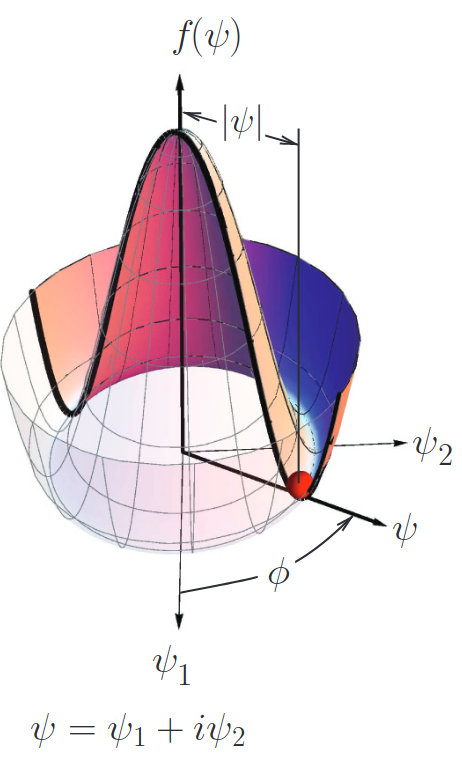
\includegraphics[width=0.3\textwidth]{images/landau free energy mexican hat}
    \caption{Mexican hat potential}
    \label{fig:Landau free energy mexican hat potential}
\end{figure}

In this `Mexican hat' potential: order parameter can be rotated continuously from one broken-symmetry state to another.
If we want the phase to be rigid, we need to introduce an
There is a topological argument for the fact that the phase is rigid.
This leads to Ginzburg-Landau theory.
Will see later: well-defined phase is associated with persistent currents or superflow.

\subsection{Ginzburg-Landau theory I: Ising order}

\todo{Short introduction for one-component order parameter, so the connection to complex order parameters gets clear}

\subsection{Ginzburg-Landau theory II: complex order and superflow}

Now: G-L theory of complex or two-component order parameters, so superfluids and superconductors.
Heart of discussion: emergence of a `macroscopic wavefunction', where the microscopic field operators \(\hat{\psi(x)}\) acquire an expectation value:
\todo{What exactly are field operators again?}
\begin{equation}
    \braket{\psi (x)} = \psi (x) = \vert \psi (x) \vert e^{\iu \theta(x)}
\end{equation}
Magnitude determines density of particles in the superfluid:
\begin{equation}
    \vert \psi(x) \vert^2 = n_s (x)
\end{equation}
\todo{More info on that? Does that come later in chapter?}
Twist/gradient of phase determines superfluid velocity:
\begin{equation}
    \vb{v}_s (x) = \frac{\hbar}{m} \Delta \phi (x)
\end{equation}
We will derive this later in the chapter.
Counterintuitive from quantum mechanics: GL suggested that \(\Phi(x)\) is a macroscopic manifestation of a macroscopic number of particles condensed into precisely the same quantum state.
Emergent phenomenon, collective properties of mater not a-priori self-evident from microscopic physics.

\todo{Here: rest of notes from Goodnotes}

\todo{Coherent states/Interpretation of states/Off-diagonal long-range order}

Phase rigidity and superflow: in GL theory, energy is sensitive to a twist of the phase.
Substitute \(\psi = \vert \psi \vert e^{\iu \phi}\) into GL free energy, gradient term is:
\begin{equation}
    \Delta \psi = ()
\end{equation}

\todo{Here: particle-current operator, especially for coherent state, connection with phase twist}

\subsection{Ginzburg-Landau theory III: charged fields}

\todo{Here: Meissner effect, etc}

\end{document}

% Print the bibliography
\cleardoublepage
\phantomsection
\addcontentsline{toc}{chapter}{Bibliography}
\printbibliography

% Beginning of the backmatter
\backmatter
\end{document}
